\documentclass[11pt,letterpaper]{article}

\usepackage[T1]{fontenc}
\usepackage{lmodern}
\usepackage{microtype}
\usepackage{amsmath,amssymb}
\usepackage{graphicx}
\usepackage{booktabs}
\usepackage[margin=1in]{geometry}
\usepackage[numbers,sort&compress]{natbib}
\usepackage{xcolor}
\usepackage[font=small,labelfont=bf]{caption}
\usepackage{subcaption}
\usepackage{placeins}
\usepackage[colorlinks=true,linkcolor=blue!45!black,citecolor=blue!45!black,urlcolor=blue!55!black]{hyperref}

\graphicspath{{figures/}}
\numberwithin{equation}{section}
\renewcommand{\topfraction}{0.9}
\renewcommand{\bottomfraction}{0.8}
\renewcommand{\textfraction}{0.07}
\renewcommand{\floatpagefraction}{0.75}
\setcounter{topnumber}{3}
\setcounter{totalnumber}{4}

\title{Sedov--Taylor Expansion from a Center of Expansion Beyond the Horizon:\\
Enclosed-Mass Gravity and the Angular Pattern of the X-ray Cluster\\
$L_X$--$T$ Anisotropy}
\author{Chris}
\date{September 25, 2026}

\begin{document}
\maketitle

\begin{abstract}
We consider a cosmological model in which the observed expansion is the
interior flow of a Sedov--Taylor self-similar blast wave launched from a real
Center of Expansion (CoE) that lies beyond the observable horizon. The
observer is displaced from the CoE, the matter density is centrally
concentrated and decreases outward, and gravity is computed from the enclosed
mass via Gauss's law, $g=-GM(<r)/r^2$. Purely homologous expansion yields an
isotropic apparent Hubble law for every observer, independent of position;
direction dependence therefore arises only through the gravitational
deceleration of the flow in the radially decreasing density profile. At
leading order in the ratio of source depth to CoE distance the induced sky
pattern is a quadrupole about the CoE axis, with a natural amplitude set by
$\kappa=\Omega_m/2$. We compare the predicted angular pattern with the
longitude dependence of the normalization $A$ of the X-ray cluster $L_X$--$T$
relation reported by Migkas et al.\ (2020). An empirical dipole-plus-quadrupole
description of the digitized $A(\ell)$ profile attains $R^2=0.814$, compared
with $R^2=0.271$ for a dipole alone. The axisymmetric Sedov--Taylor/Gauss
geometry attains $R^2=0.307$; with a phase-rotation template and a
multiplicative second-harmonic correction the agreement reaches $R^2=0.875$.
The four extrema of the corrected profile, mapped onto the sky as small circles
about a CoE axis tilted by $15^\circ$ from the Galactic plane, pass close to
the published extrema of the Migkas et al.\ $A$ map. The phase-rotation and
second-harmonic terms are presently empirical templates; deriving them from
time-integrated gravity is the principal task for future work.
\end{abstract}

%======================================================================
\section{Introduction}
\label{sec:intro}

The self-similar blast wave produced by a point release of energy $E$ into a
uniform medium of density $\rho$ was obtained independently by
Sedov~\citep{Sedov1946} and Taylor~\citep{Taylor1950}. Its shock radius obeys
$R\propto(Et^2/\rho)^{1/5}$, and the solution generalizes to power-law ambient
densities and, in the ultra-relativistic regime, to the similarity solutions of
Blandford and McKee~\citep{BlandfordMcKee1976}, which constitute the relativistic
generalization of the Sedov--Taylor problem. In a cosmological setting,
Bertschinger~\citep{Bertschinger1983} found self-similar blast waves in an
Einstein--de~Sitter background whose early evolution follows the Sedov
solution before being modified by the cosmological expansion. In general
relativity, Smoller and Temple~\citep{SmollerTemple2000,SmollerTemple2003}
constructed exact solutions of the Einstein equations in which a
Friedmann--Robertson--Walker expansion emerges behind a shock wave at the
leading edge of a large-scale explosion, with the shock located at or beyond
one Hubble length and, in the latter case, inside a black hole.

These works motivate a class of models in which the observed Hubble expansion
is the interior flow of an explosion about a physical center, rather than a
homogeneous expansion without a center. In such a model the observer is, in
general, not located at the center, and the question arises whether the
resulting departures from isotropy are observable.

A candidate observable is the anisotropy of galaxy-cluster scaling relations
reported by Migkas et al.~\citep{Migkas2020}. Using 313 clusters from the
Meta-Catalogue of X-ray detected Clusters of galaxies, these authors found that
the normalization $A$ of the $L_X$--$T$ relation depends on sky direction, with
anisotropy at the $\gtrsim4\sigma$ level toward Galactic coordinates
$(\ell,b)\sim(280^\circ,-20^\circ)$. Since $L_X$ depends on the assumed luminosity
distance while the spectroscopic temperature does not, a direction-dependent
$A$ can be interpreted as a direction-dependent distance--redshift relation.

In this paper we formulate a Sedov--Taylor model with an off-center observer,
a centrally concentrated density profile, and enclosed-mass gravity
(Section~\ref{sec:model}); describe the comparison with the Migkas et al.\
longitude profile $A(\ell)$ and sky map (Section~\ref{sec:methods}); present
the resulting fits and sky geometry (Section~\ref{sec:results}); and discuss
the status and limitations of the comparison (Section~\ref{sec:discussion}).

%======================================================================
\section{Model}
\label{sec:model}

\subsection{Dynamics: Sedov--Taylor self-similar expansion}
\label{sec:dynamics}

We take the expansion to be the interior of a Sedov--Taylor blast wave centered
on the CoE. For energy $E$ released into a uniform medium of density $\rho$,
dimensional analysis and self-similarity give the shock radius
\begin{equation}
  R(t) = \xi_0\left(\frac{E\,t^2}{\rho}\right)^{1/5},
  \label{eq:ST}
\end{equation}
where $\xi_0$ is a dimensionless constant of order unity that depends on the
adiabatic index~\citep{Sedov1946,Taylor1950}. For a centrally concentrated
medium whose density decreases as a power law,
\begin{equation}
  \rho(r) = \rho_1\left(\frac{r}{r_1}\right)^{-w},
  \label{eq:rhow}
\end{equation}
the same argument, with $\rho_1 r_1^{w}$ replacing $\rho$ as the dimensional
parameter, gives
\begin{equation}
  R(t) = \xi_w\left(\frac{E\,t^2}{\rho_1 r_1^{w}}\right)^{1/(5-w)}
  \;\propto\; t^{2/(5-w)},
  \qquad w<5 ,
  \label{eq:STw}
\end{equation}
which reduces to Eq.~\eqref{eq:ST} for $w=0$. The shock velocity is
$\dot R=[2/(5-w)]\,R/t$, so that the expansion rate at the shock is
\begin{equation}
  H(t) \equiv \frac{\dot R}{R} = \frac{2}{(5-w)\,t}.
  \label{eq:Hst}
\end{equation}
The corresponding relativistic self-similar solutions, including ambient
densities varying with radius, were given by Blandford and
McKee~\citep{BlandfordMcKee1976}; cosmological and general-relativistic
analogues are those of Bertschinger~\citep{Bertschinger1983} and of Smoller and
Temple~\citep{SmollerTemple2000,SmollerTemple2003}.

In the interior of the blast we adopt the homologous approximation, in which
every fluid element moves radially away from the CoE with a velocity
proportional to its distance,
\begin{equation}
  \vec v(\vec R) = H\,\vec R .
  \label{eq:homology}
\end{equation}
Let the observer $O$ be located at $\vec R_O$ and a source $P$ at $\vec R_P$.
The relative velocity is
\begin{equation}
  \vec v_{\mathrm{rel}} = \vec v_P - \vec v_O = H\,(\vec R_P-\vec R_O) = H\,\vec d,
  \label{eq:vrel}
\end{equation}
where $\vec d$ is the observer--source separation. The line-of-sight recession
velocity is $v_{\mathrm{los}}=\vec v_{\mathrm{rel}}\cdot\hat d=H d$, so that
\begin{equation}
  H_{\mathrm{obs}} \equiv \frac{v_{\mathrm{los}}}{d} = H
  \label{eq:Hobs}
\end{equation}
in every direction. The position of the CoE therefore drops out of all relative
velocities (Fig.~\ref{fig:homology}): an off-center observer in a purely
homologous flow measures an isotropic Hubble law. Any observable anisotropy
must arise from a departure from homology, which in the present model is
supplied by gravity.

\begin{figure}[!htbp]
\centering
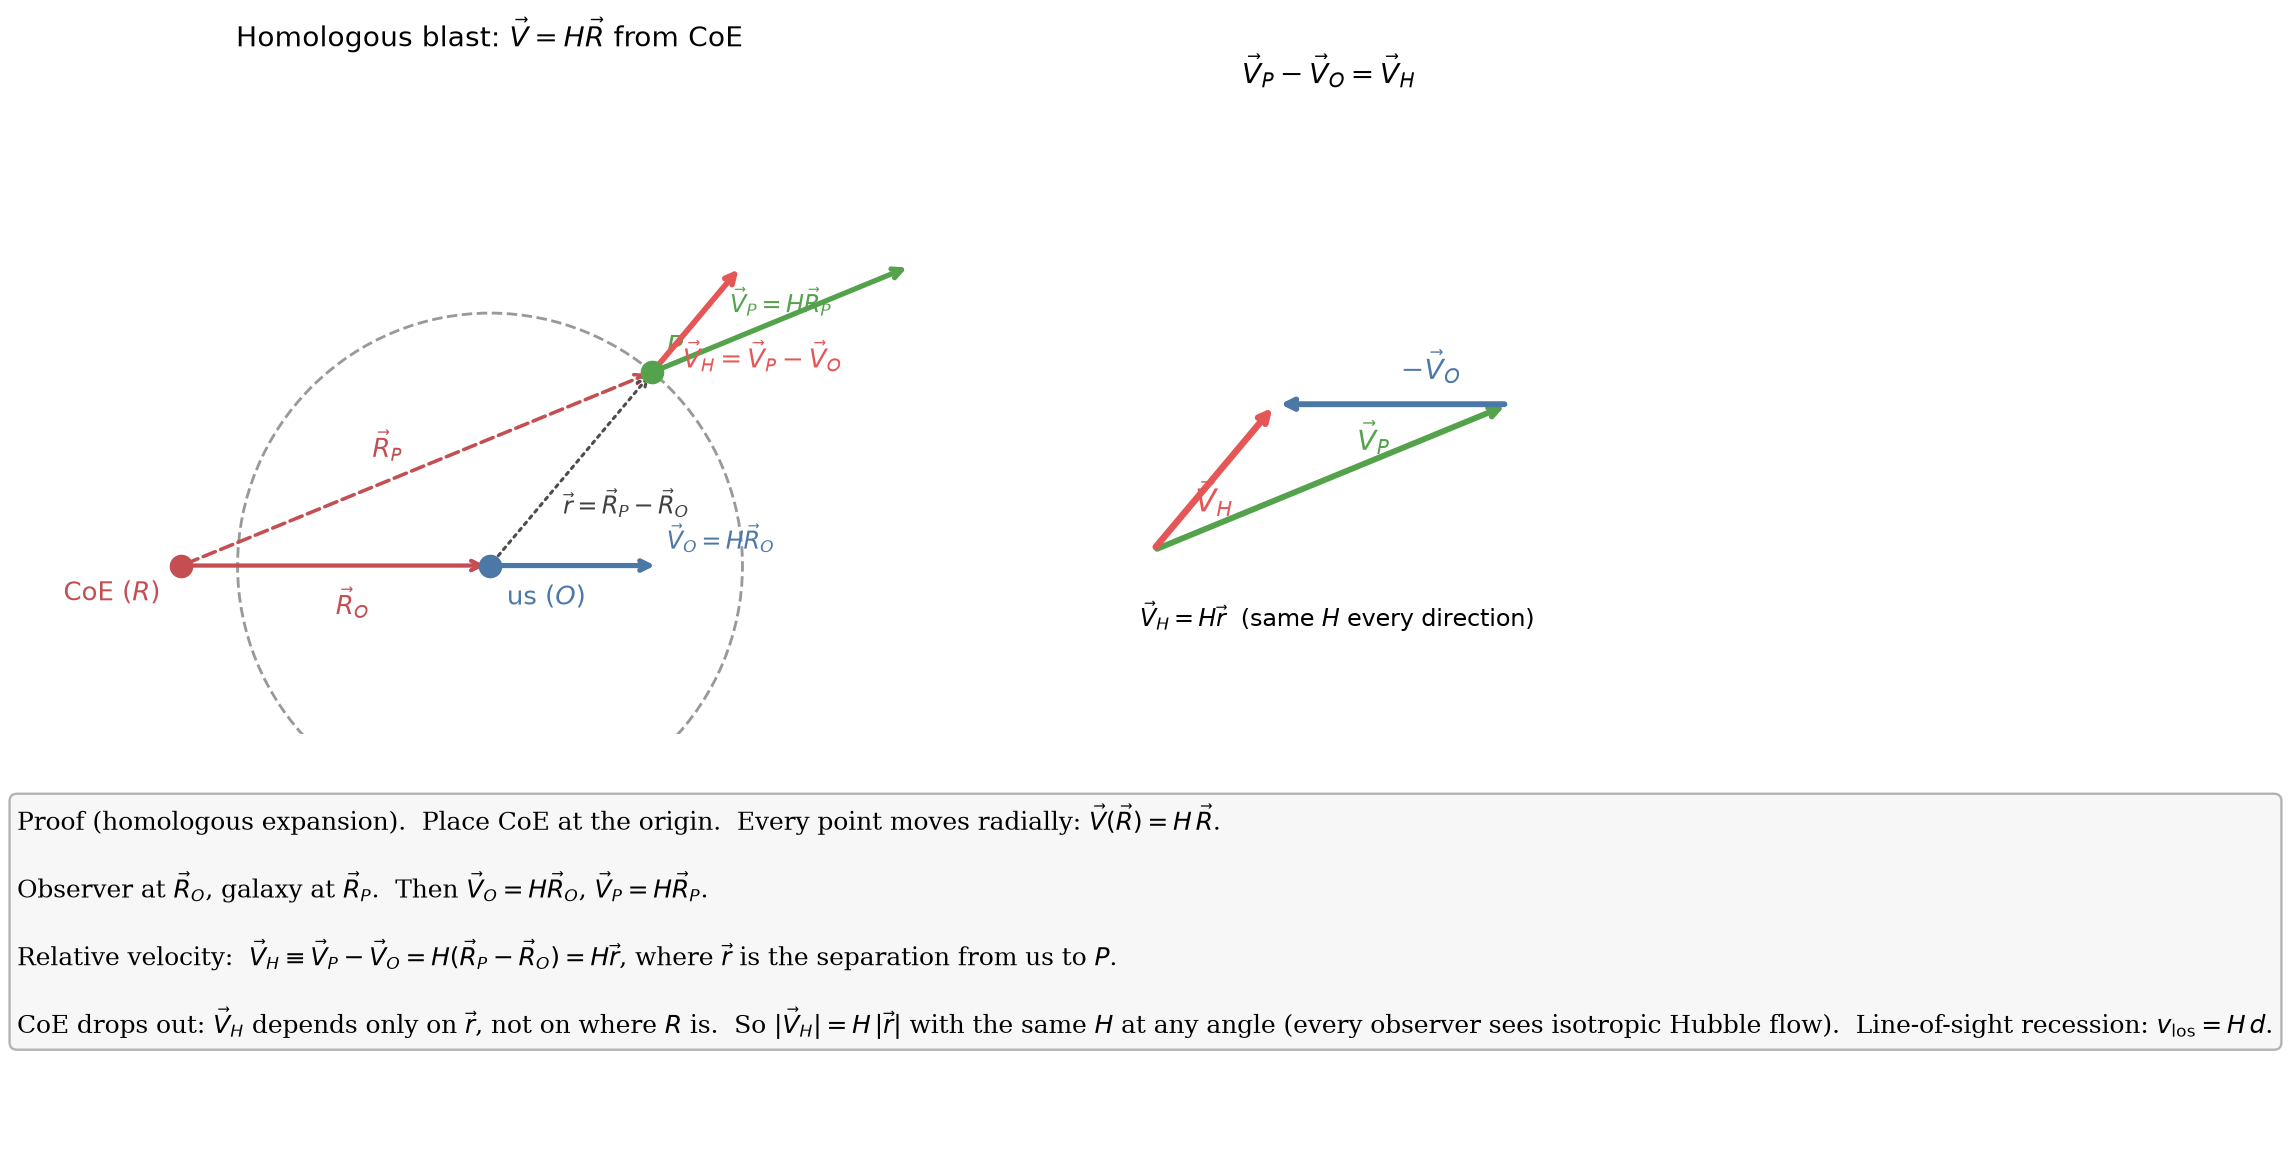
\includegraphics[width=\textwidth]{hubble_from_coe_relative_velocity.png}
\caption{Homologous expansion about the CoE. Absolute velocities
$\vec V=H\vec R$ are directed radially away from the CoE, but the velocity of a
source $P$ relative to the observer $O$ is $H(\vec R_P-\vec R_O)$, which depends
only on the separation. Every observer therefore measures the same isotropic
expansion rate $H$, irrespective of its distance from the CoE
(Eqs.~\ref{eq:homology}--\ref{eq:Hobs}).}
\label{fig:homology}
\end{figure}

\subsection{Geometry}
\label{sec:geometry}

The CoE is placed at the origin and lies beyond the observer's horizon. The
observer is at distance $D$ from the CoE along the unit vector $\hat D$, and
sources are located at observer-centric distance $d$ in direction $\hat n$, so
that the source position relative to the CoE is $\vec r=\vec D+d\,\hat n$
(Fig.~\ref{fig:geometry}). We write
\begin{equation}
  \mu \equiv \hat n\cdot\hat D = \cos\phi ,
  \label{eq:mu}
\end{equation}
where $\phi$ is the sky angle measured from the anti-CoE direction ($\phi=0$)
toward the CoE ($\phi=180^\circ$). The relevant expansion parameter is $d/D$,
which is small for survey depths much less than the distance to the CoE.

\begin{figure}[!htbp]
\centering
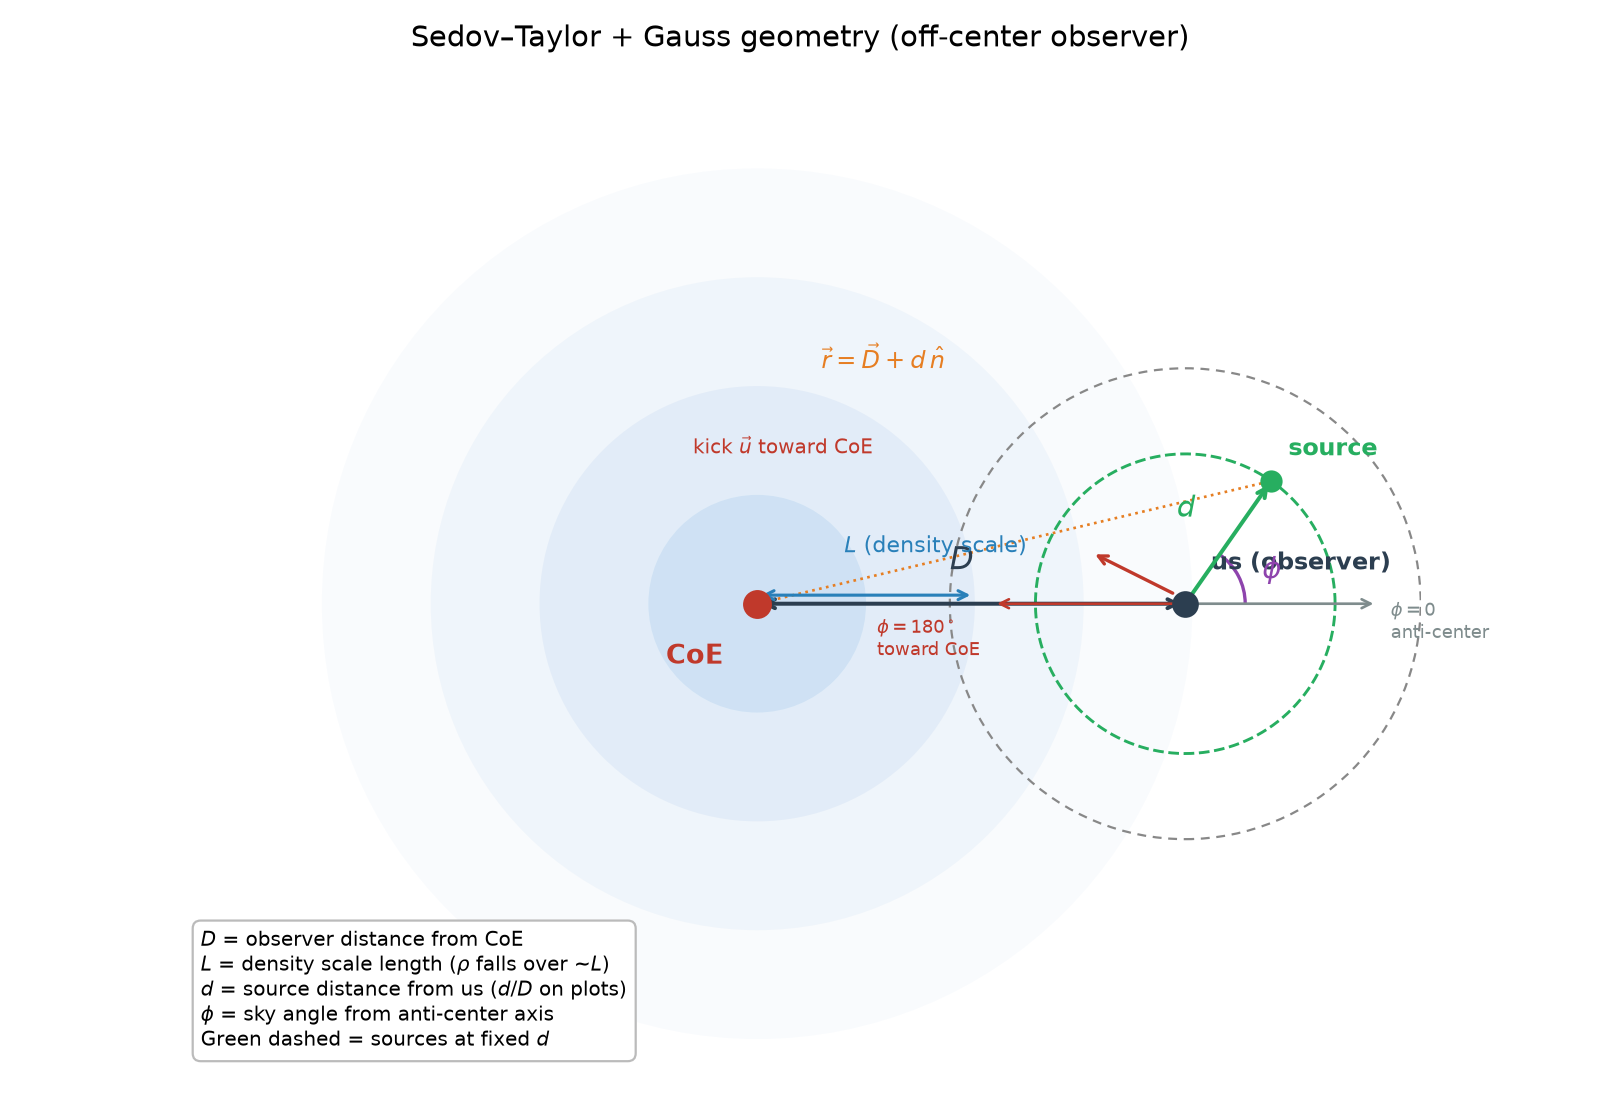
\includegraphics[width=0.78\textwidth]{geometry_CoE_observer.png}
\caption{Model geometry. The CoE lies at the origin, embedded in a centrally
concentrated density distribution with scale length $L$. The observer is at
distance $D$ from the CoE; sources lie at observer-centric distance $d$ and
sky angle $\phi$ measured from the anti-CoE direction.}
\label{fig:geometry}
\end{figure}

\subsection{Density profile}
\label{sec:density}

A uniform-density sphere produces an interior gravitational acceleration
$\vec g\propto-\vec r$, which is itself homologous; it decelerates the flow
uniformly and cannot generate direction dependence in $H_{\mathrm{obs}}$. We
therefore adopt a spherically symmetric, centrally concentrated profile that
decreases outward. For the calculations presented here we use the exponential
profile
\begin{equation}
  \frac{\rho(r)}{\rho_0} = e^{-r/L},
  \label{eq:rhoexp}
\end{equation}
whose local logarithmic slope $w_{\mathrm{eff}}=-\,d\ln\rho/d\ln r=r/L$ increases
outward, connecting to the power-law scaling of Eq.~\eqref{eq:STw}. The
enclosed-mass fraction, with $X\equiv r/L$ and $M$ the total mass, is
\begin{equation}
  \frac{M(<r)}{M} = 1 - e^{-X}\left(1+X+\tfrac12 X^2\right),
  \label{eq:menc}
\end{equation}
obtained by integrating $4\pi r^2\rho(r)$. Both functions are shown in
Fig.~\ref{fig:density}.

\begin{figure}[!htbp]
\centering
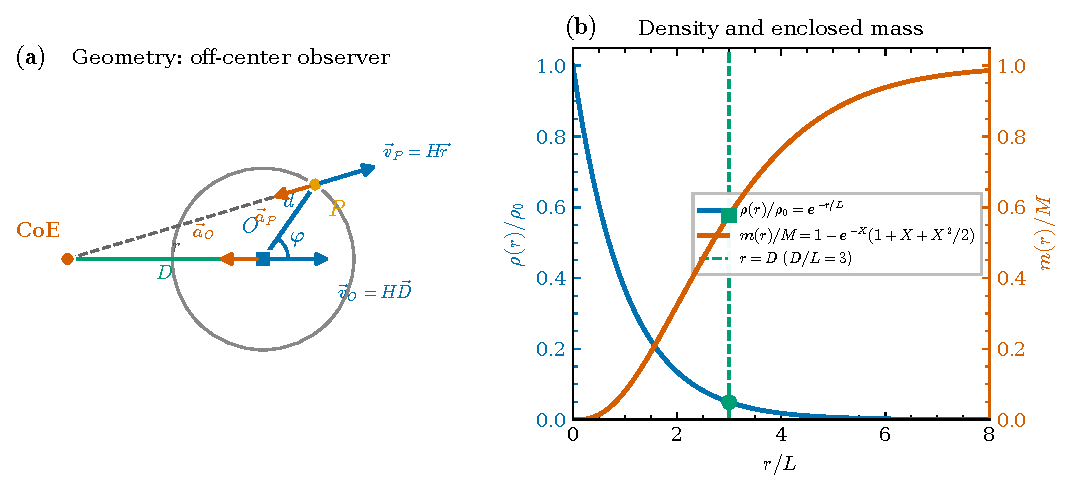
\includegraphics[width=0.92\textwidth]{sedov_decreasing_density_toy_journal.pdf}
\caption{Centrally concentrated density profile used in the model. Left:
exponential density $\rho(r)/\rho_0=e^{-r/L}$ (Eq.~\ref{eq:rhoexp}). Right:
enclosed-mass fraction $M(<r)/M$ (Eq.~\ref{eq:menc}). The vertical marker
indicates an illustrative observer distance $D/L=3$.}
\label{fig:density}
\end{figure}

\subsection{Gravity}
\label{sec:gravity}

For a spherically symmetric mass distribution, Gauss's law gives the
gravitational acceleration at radius $r$ from the CoE in terms of the enclosed
mass alone,
\begin{equation}
  \vec g(r) = -\frac{G\,M(<r)}{r^2}\,\hat r .
  \label{eq:gauss}
\end{equation}
Because $M(<r)/r^3$ decreases outward for the profile of
Eq.~\eqref{eq:rhoexp}, sources closer to and farther from the CoE than the
observer are decelerated by different amounts relative to the observer, which
breaks the homology of Eq.~\eqref{eq:homology}. A natural dimensionless
measure of the gravitational strength at the observer is
\begin{equation}
  \kappa \equiv \frac{G\,M(<D)}{D^3 H^2}
  = \frac{4\pi G\bar\rho(<D)}{3H^2}
  = \frac{\Omega_m}{2},
  \label{eq:kappa}
\end{equation}
where $\bar\rho(<D)$ is the mean density within $D$ and
$\Omega_m=8\pi G\bar\rho/(3H^2)$. For $\Omega_m=0.3$ this gives
$\kappa_{\mathrm{nat}}=0.15$.

Expanding the relative gravitational acceleration between source and observer
to leading orders in $d/D$ gives the tidal form
\begin{equation}
  \frac{H_{\mathrm{obs}}(\hat n)}{H} - 1
  \simeq \alpha\kappa\,(3\mu^2-1)
  + \alpha\kappa\,\frac{d}{D}\left(\tfrac{9}{2}\mu - \tfrac{15}{2}\mu^3\right),
  \label{eq:tidal}
\end{equation}
where $\alpha$ is an order-unity coefficient that depends on how the
acceleration is integrated along the flow. The leading term is a quadrupole,
$3\mu^2-1=2P_2(\mu)$, with Legendre coefficient $C_2\simeq2\alpha\kappa$
($C_2\simeq0.30$ for $\alpha=1$, $\kappa=0.15$), while the full-sky dipole
coefficient $C_1$ vanishes at this order; the first odd contribution is an
octupole of relative size $\mathcal O(d/D)$. A spherically symmetric
enclosed-mass model with a distant CoE therefore predicts a sky pattern that is
axisymmetric about $\hat D$ and quadrupole-dominated.

%======================================================================
\section{Methods: comparison with Migkas et al.\ (2020)}
\label{sec:methods}

\subsection{Observational target}

Migkas et al.~\citep{Migkas2020} report the $L_X$--$T$ normalization $A$,
relative to its all-sky value $A_{\mathrm{all}}$, as a function of Galactic
longitude in sliding longitude sectors (their Fig.~6), and as a full-sky map of
$A/A_{\mathrm{all}}$ from cones of opening angle $\theta=75^\circ$ (their Fig.~8).
We digitized the longitude profile at $71$ longitudes spaced by $5^\circ$
($\ell=5^\circ,\dots,355^\circ$). For the sky comparison we use the extrema of the
$\theta=75^\circ$ map: the highest normalization near $(\ell,b)=(17^\circ,-9^\circ)$
and the lowest near $(274^\circ,-22^\circ)$~\citep{Migkas2020}.

As an empirical characterization of the digitized profile, a linear
least-squares fit of a monopole plus dipole in longitude gives $R^2=0.271$,
whereas adding the second harmonic,
\begin{equation}
  \frac{A(\ell)}{A_{\mathrm{all}}}
  = 0.997 + 0.030\cos\ell + 0.043\sin\ell + 0.064\cos2\ell + 0.037\sin2\ell ,
  \label{eq:dq}
\end{equation}
gives $R^2=0.814$ and an rms residual of $0.031$ (Fig.~\ref{fig:dq}). The
second harmonic is thus the dominant angular structure of the profile,
consistent in character with the quadrupole predicted by
Eq.~\eqref{eq:tidal}.

\begin{figure}[!htbp]
\centering
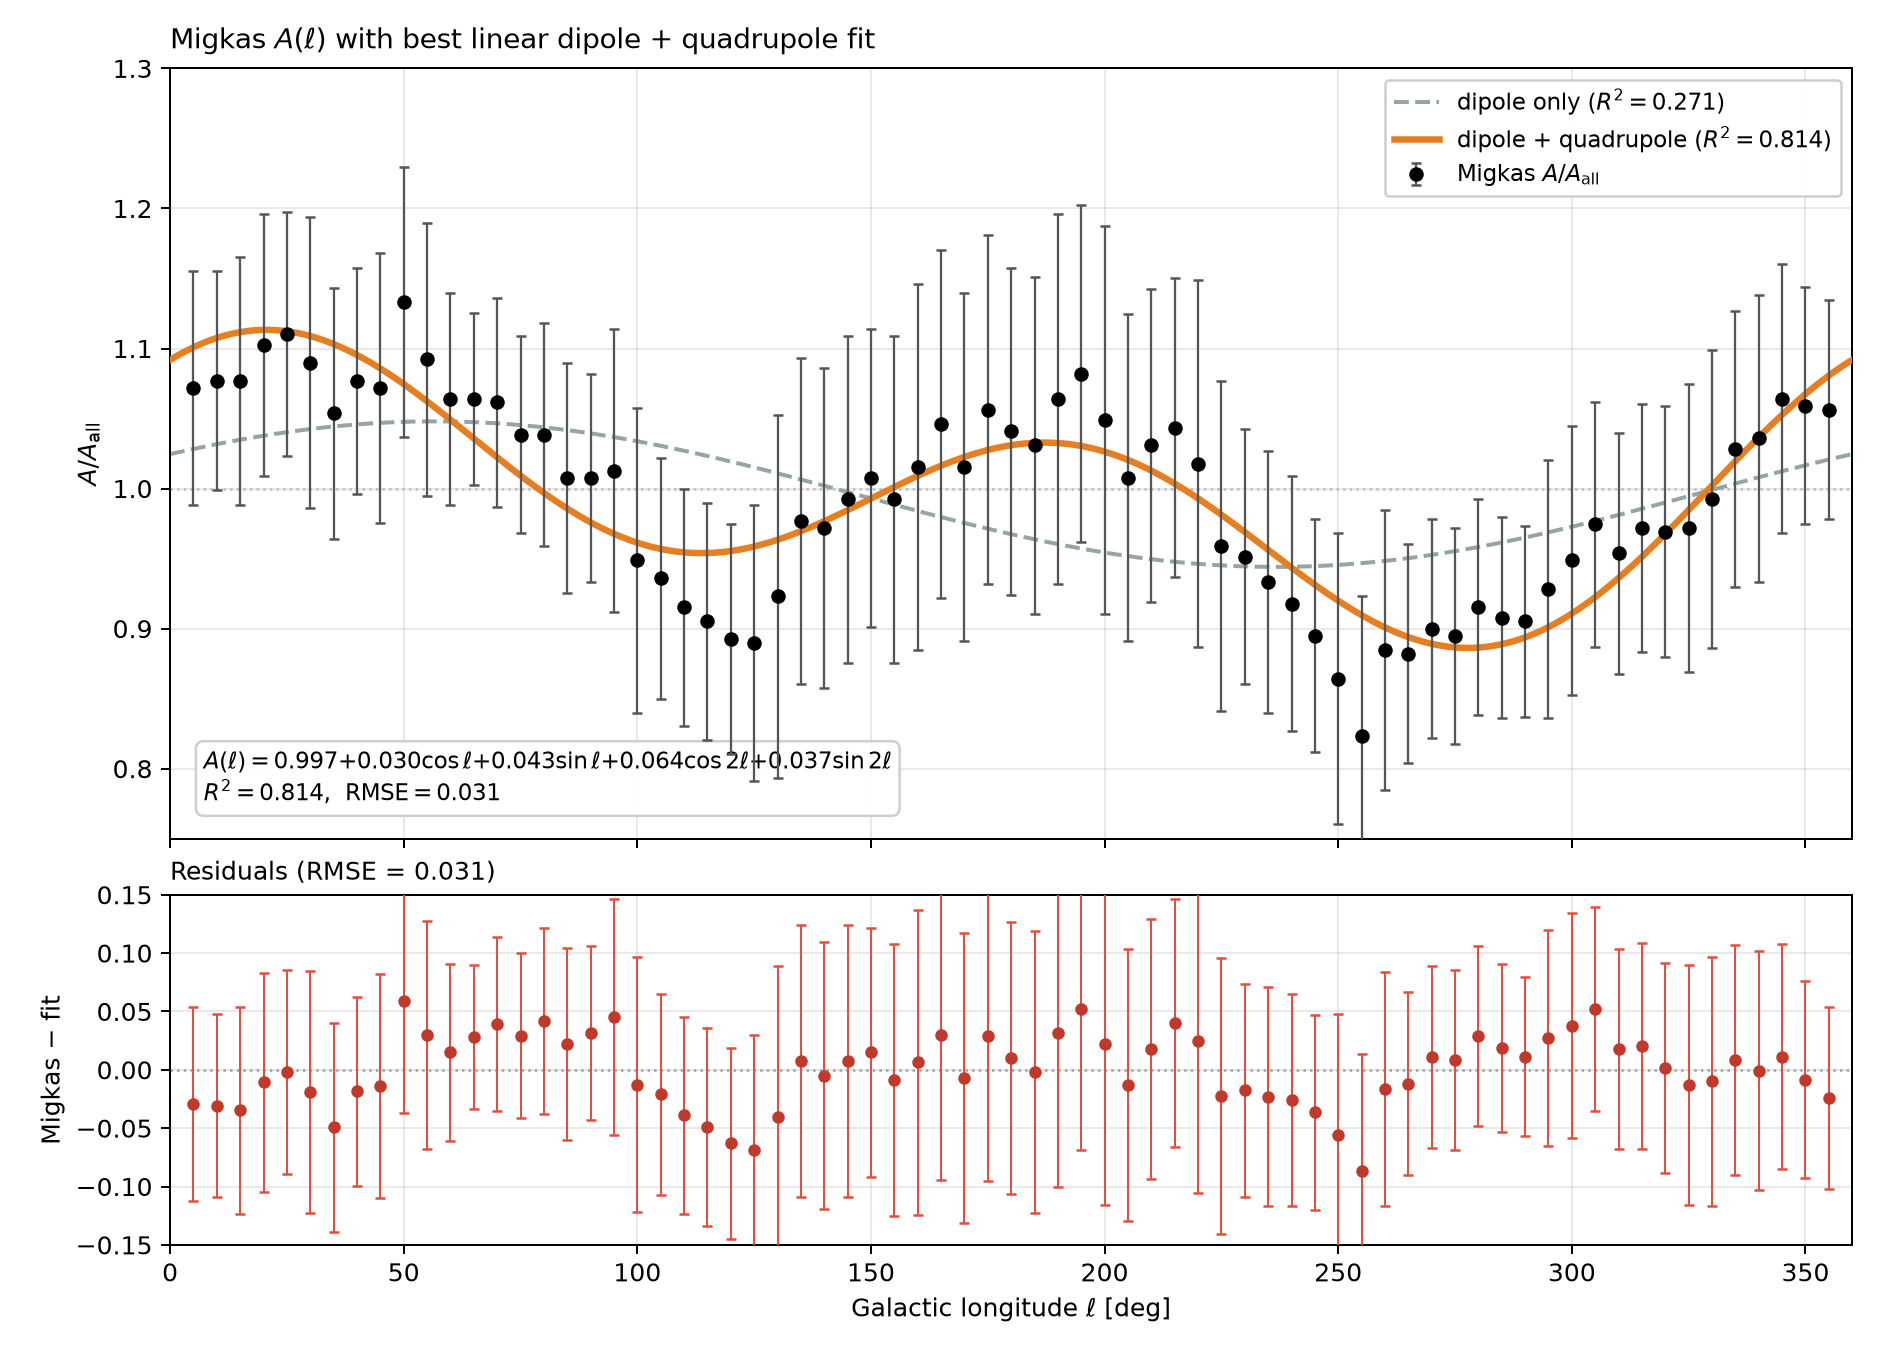
\includegraphics[width=0.85\textwidth]{migkas_dipole_quadrupole_fit.png}
\caption{Digitized longitude profile $A/A_{\mathrm{all}}$ of Migkas et
al.~\citep{Migkas2020} (points with error bars) with linear least-squares fits.
Dashed: monopole plus dipole, $R^2=0.271$. Solid: monopole plus dipole plus
quadrupole (Eq.~\ref{eq:dq}), $R^2=0.814$, rms residual $0.031$. Lower panel:
residuals of the dipole-plus-quadrupole fit.}
\label{fig:dq}
\end{figure}

\subsection{Model observable}

The model predicts $H_{\mathrm{obs}}(\hat n)/H$. We map this onto the
normalization through
\begin{equation}
  \frac{A}{A_{\mathrm{all}}} \;\propto\; \frac{H_{\mathrm{obs}}}{H},
  \label{eq:Aproxy}
\end{equation}
renormalized to unit mean over the longitude strip. The model profile is
evaluated along the Galactic plane, with the angle $\phi$ of
Eq.~\eqref{eq:mu} related to Galactic longitude by the orientation of the CoE
axis.

\subsection{Phase-rotation and second-harmonic templates}

Two empirical corrections are applied to the axisymmetric model profile
$A_{\mathrm{phys}}(\ell)$. The first is a phase-rotation template,
\begin{equation}
  A'(\ell) = \bigl[1-\mathrm{Amp}\,\sin(\Omega\ell+\varphi)\bigr]\,A_{\mathrm{phys}}(\ell),
  \qquad \Omega=\frac{2\pi}{360^\circ},
  \label{eq:ampsin}
\end{equation}
with amplitude $\mathrm{Amp}$ and phase $\varphi$ scanned on a grid. The second
is a multiplicative second-harmonic correction,
\begin{equation}
  A_{\mathrm{c}}(\ell) = \bigl[1+\varepsilon\,\sin(2\ell+\psi)\bigr]\,A'(\ell),
  \label{eq:2ell}
\end{equation}
with $\varepsilon$ and $\psi$ fitted to the residuals. Goodness of fit is
reported as the coefficient of determination $R^2$ against the digitized
profile, together with the rms residual.

\subsection{Sky mapping of extrema}

The extrema of the corrected profile $A_{\mathrm{c}}(\ell)$ define four angles
$\theta$, measured from the anti-CoE direction in the model frame. Because the
model is axisymmetric about $\hat D$, each angle corresponds on the sky to a
small circle (ring) of constant angular distance from the anti-CoE direction.
Each ring is drawn with a band of half-width $\pm9^\circ$ ($18^\circ$ end to end,
i.e.\ $5\%$ of $360^\circ$). The CoE axis is tilted by $+15^\circ$ out of the
Galactic plane: the anti-CoE direction is at $(\ell,b)=(0^\circ,+15^\circ)$ and the
CoE at $(180^\circ,-15^\circ)$. Sky maps use the Galactic Mollweide projection with
longitude increasing to the left, as in Migkas et al.\ Fig.~8.

%======================================================================
\section{Results}
\label{sec:results}

\subsection{Longitude profile}

Figure~\ref{fig:AF} shows the model profile obtained by integrating the
enclosed-mass acceleration along the flow for $d/D=0.1$, compared with a
single impulsive approximation and with the digitized data. The model
reproduces the two-maxima, two-minima structure of the data, but with extrema
at $\phi\simeq0^\circ,180^\circ$ and $90^\circ,270^\circ$ fixed by axisymmetry. The
axisymmetric model profile attains $R^2=0.307$ (rms residual $0.059$), and a
smooth sine-rotation of the same profile raises this to $R^2=0.553$ (rms
$0.047$; Fig.~\ref{fig:axisym}). An alternative evaluation of the first-principles geometry without any
rotation template gives $R^2=0.543$.

The phase-rotation template of Eq.~\eqref{eq:ampsin} attains its best agreement
at $\mathrm{Amp}=-0.06$, $\varphi\simeq11.5^\circ$, with $R^2=0.746$ (rms $0.038$).
The dependence of $R^2_A$ on the template parameters is shown in
Fig.~\ref{fig:heatmaps}(a): the agreement forms a broad ridge at
$\mathrm{Amp}\approx-0.04$ to $-0.08$ and $\varphi\lesssim30^\circ$, and degrades
steadily toward larger phases. Applying the same template to the slope $B$ of
the $L_X$--$T$ relation with an independent amplitude $\mathrm{Amp}_B$
[Fig.~\ref{fig:heatmaps}(b)] gives a best fit of $R^2_B=0.790$ at
$\mathrm{Amp}_B=-0.06$, $\varphi\simeq185^\circ$; the nearly equivalent solution
$\mathrm{Amp}_B=+0.06$ at small phase ($R^2_B=0.790$) corresponds to
$\mathrm{Amp}_B=-\mathrm{Amp}_A$ at the phase preferred by $A$.
Adding the second-harmonic correction of Eq.~\eqref{eq:2ell} with
$\varepsilon=-0.043$ and $\psi=175.8^\circ$ yields $R^2=0.875$ and an rms residual
of $0.029$ (Fig.~\ref{fig:2ell}). The corrected profile has maxima at
$\theta\simeq30^\circ$ and $185^\circ$ and minima at $\theta\simeq115^\circ$ and
$265^\circ$.

To isolate the contribution of the geometry, Fig.~\ref{fig:resonly} compares
the fully corrected profile with the product of the two correction factors
applied to a constant, $A=1\times F_{\mathrm{rot}}\times F_{2\ell}$, where
$F_{\mathrm{rot}}$ is the ratio of the rotated to the unrotated axisymmetric
profile and $F_{2\ell}$ is the factor of Eq.~\eqref{eq:2ell}. The squared
correlation with the data is $0.366$ for the correction factors alone and
$0.875$ for the full model. The correction factors on their own therefore do
not account for the observed profile; the axisymmetric Sedov--Taylor/Gauss
geometry carries most of the explained variance.

\begin{figure}[!htbp]
\centering
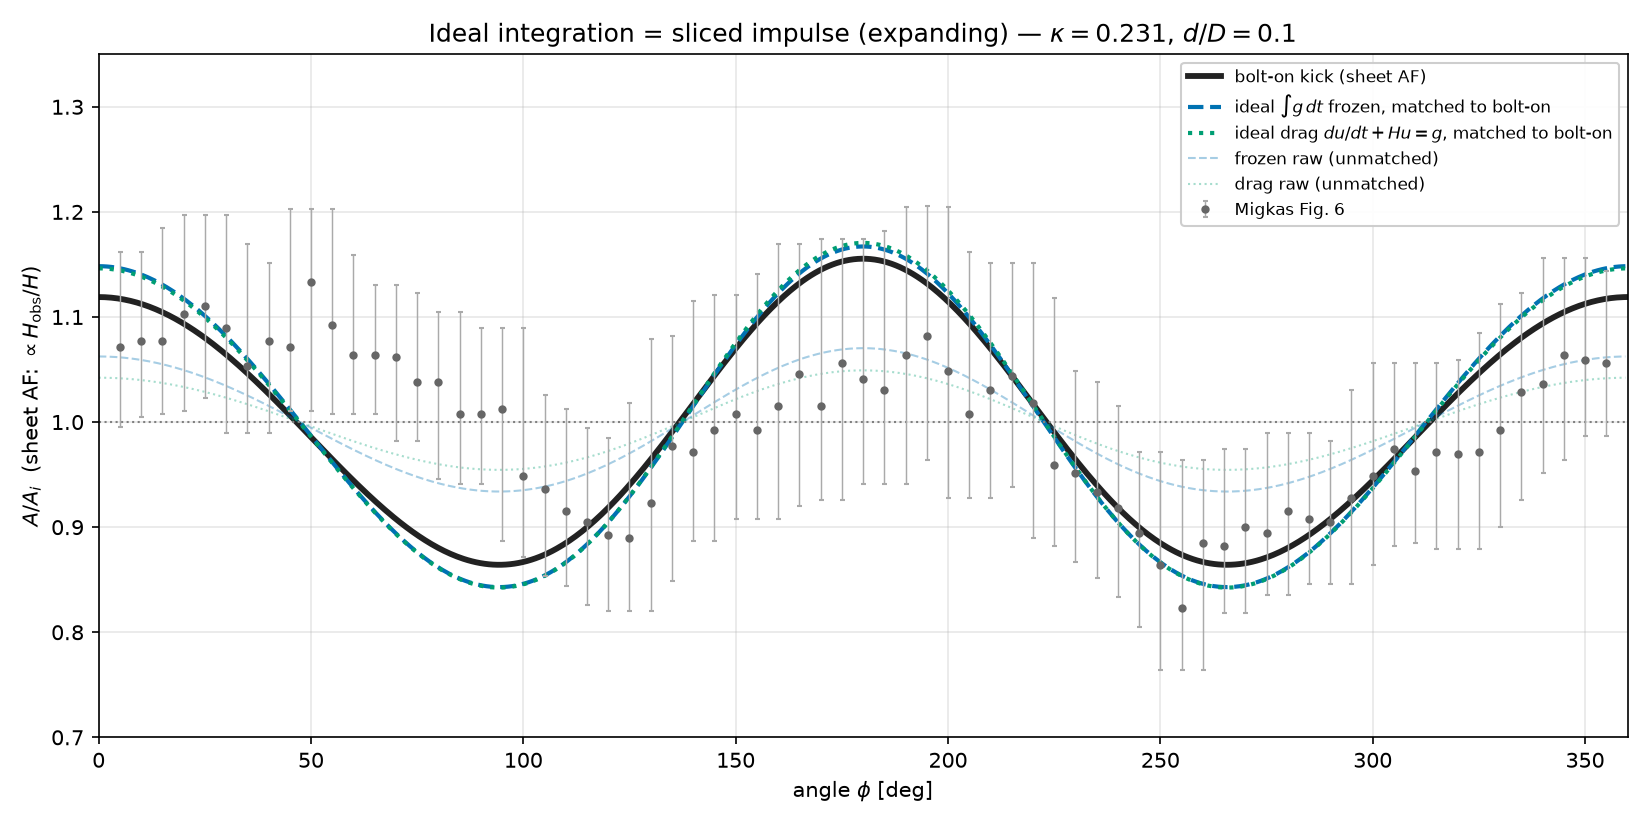
\includegraphics[width=\textwidth]{A_vs_angle_ideal_integration_sheet_AF.png}
\caption{Model $A/A_{\mathrm{all}}\propto H_{\mathrm{obs}}/H$ versus sky angle
$\phi$ for $d/D=0.1$ and $\kappa=0.231$. Solid: single impulsive deceleration.
Dashed and dotted: time-integrated enclosed-mass acceleration (frozen and
drag-coupled integration, respectively), normalized to the same amplitude;
light curves show the unnormalized integrations. Points: digitized Migkas et
al.\ profile.}
\label{fig:AF}
\end{figure}

\begin{figure}[!htbp]
\centering
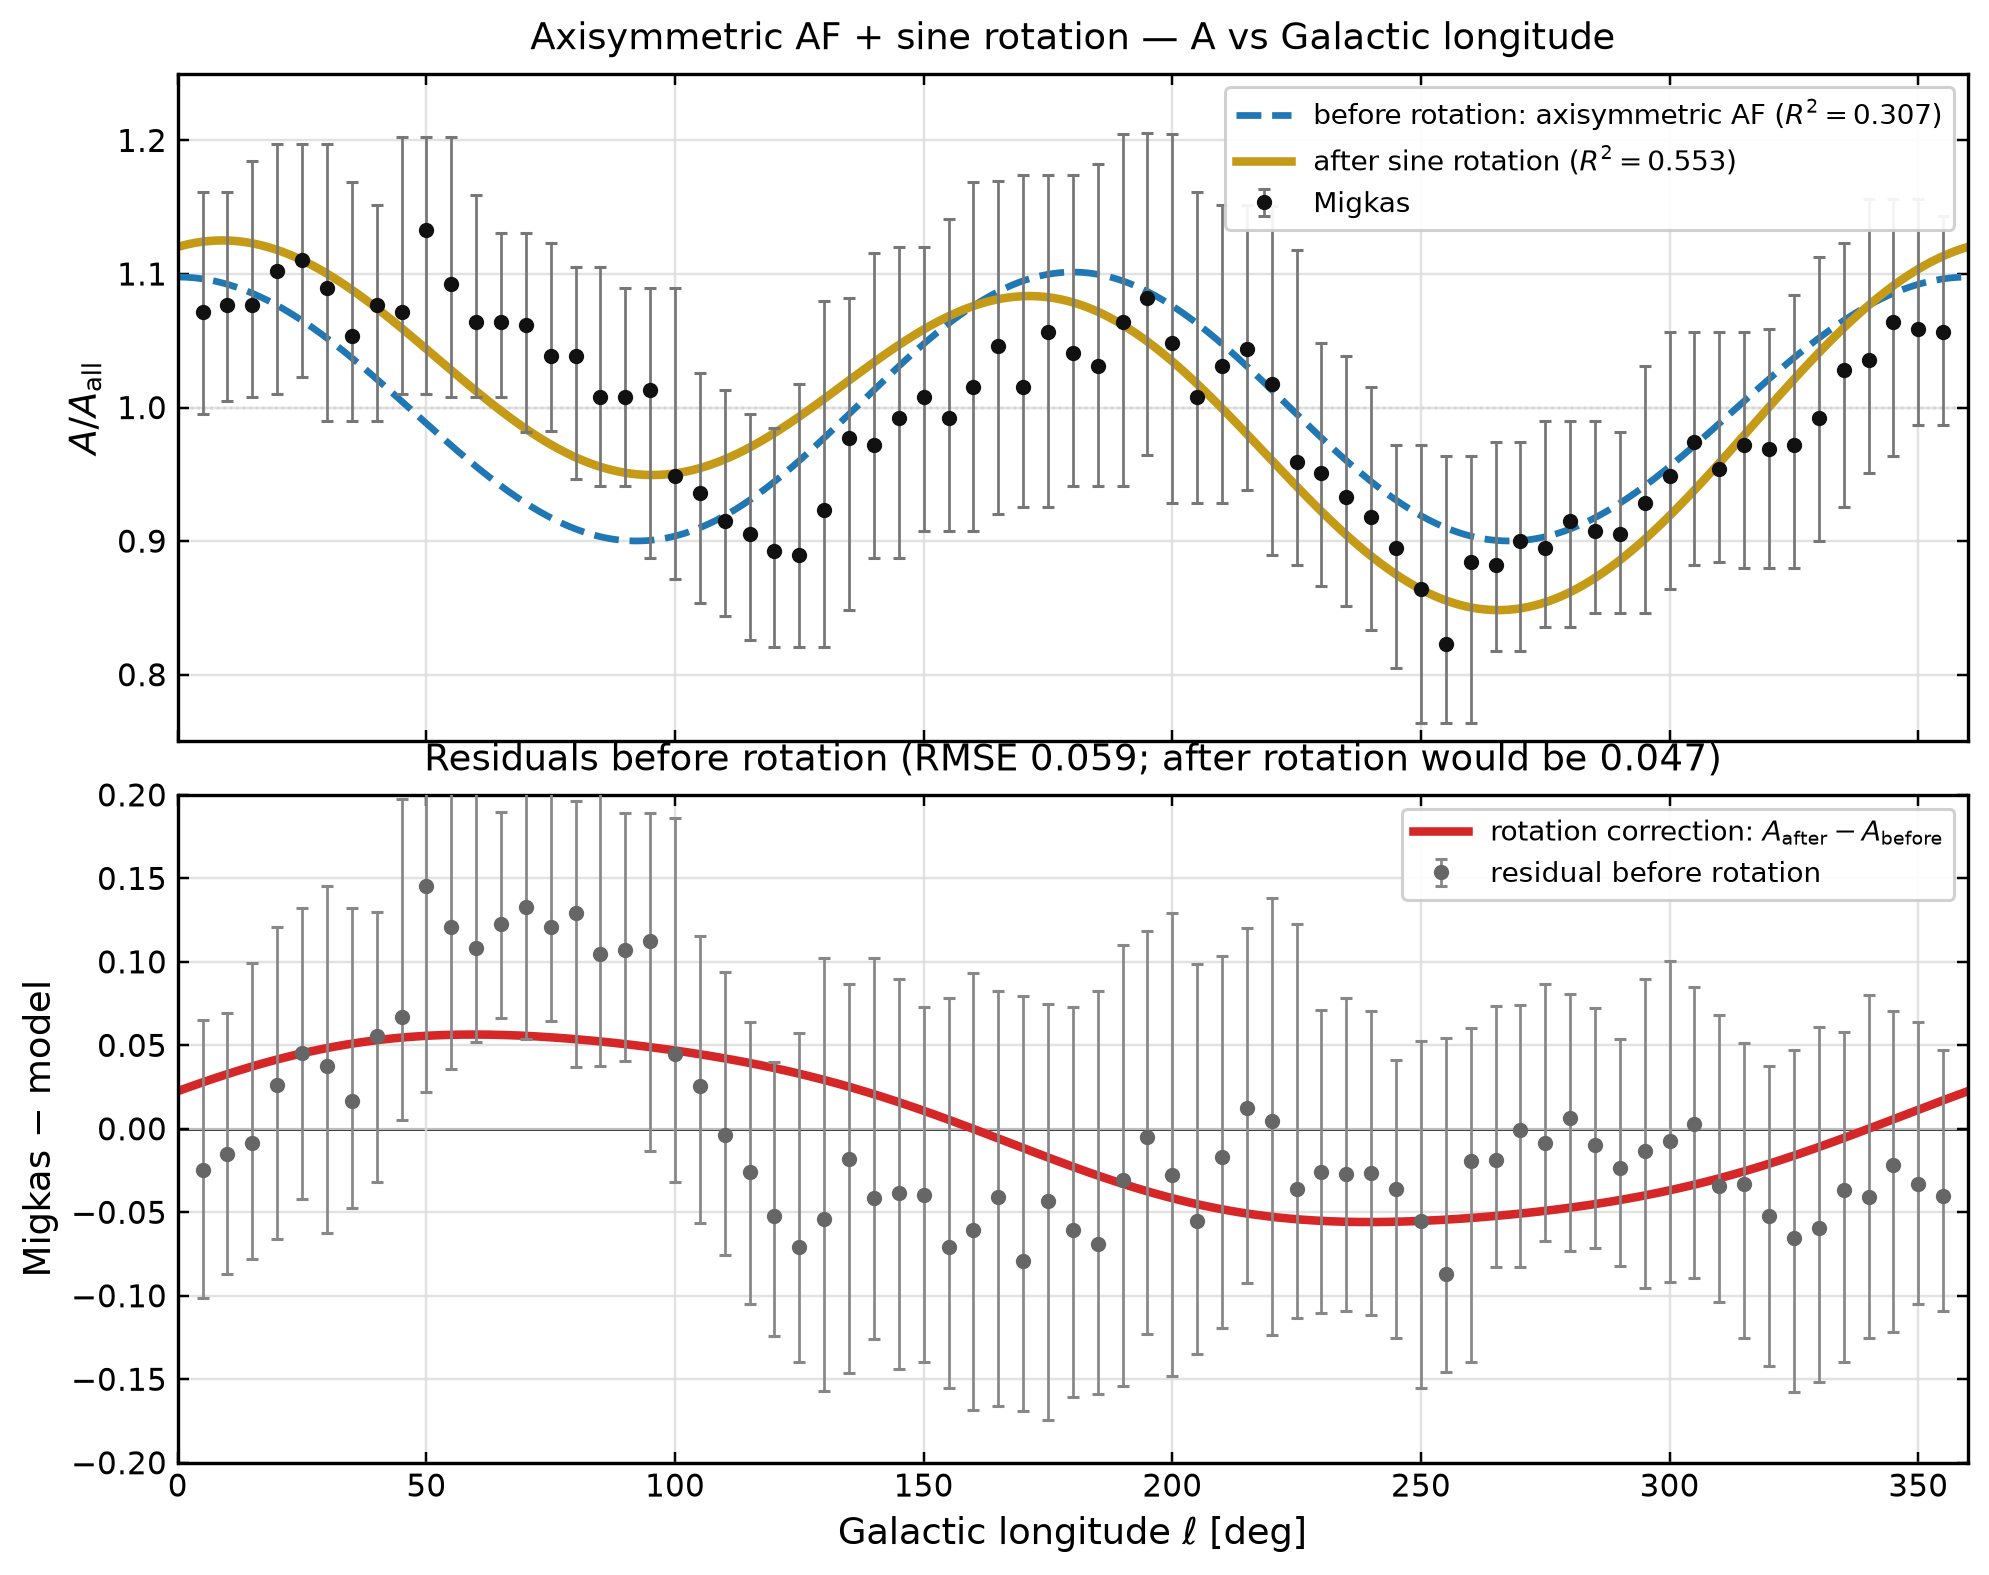
\includegraphics[width=0.85\textwidth]{A_vs_angle_axisymmetric_before_rotation_with_residuals.png}
\caption{Axisymmetric model profile versus Galactic longitude before (dashed,
$R^2=0.307$) and after (solid, $R^2=0.553$) a smooth sine rotation, compared with
the digitized Migkas et al.\ profile. Lower panel: residuals before rotation
(rms $0.059$) and the rotation correction $A_{\mathrm{after}}-A_{\mathrm{before}}$.}
\label{fig:axisym}
\end{figure}

\begin{figure}[!htbp]
\centering
\begin{subfigure}[t]{0.495\textwidth}
  \centering
  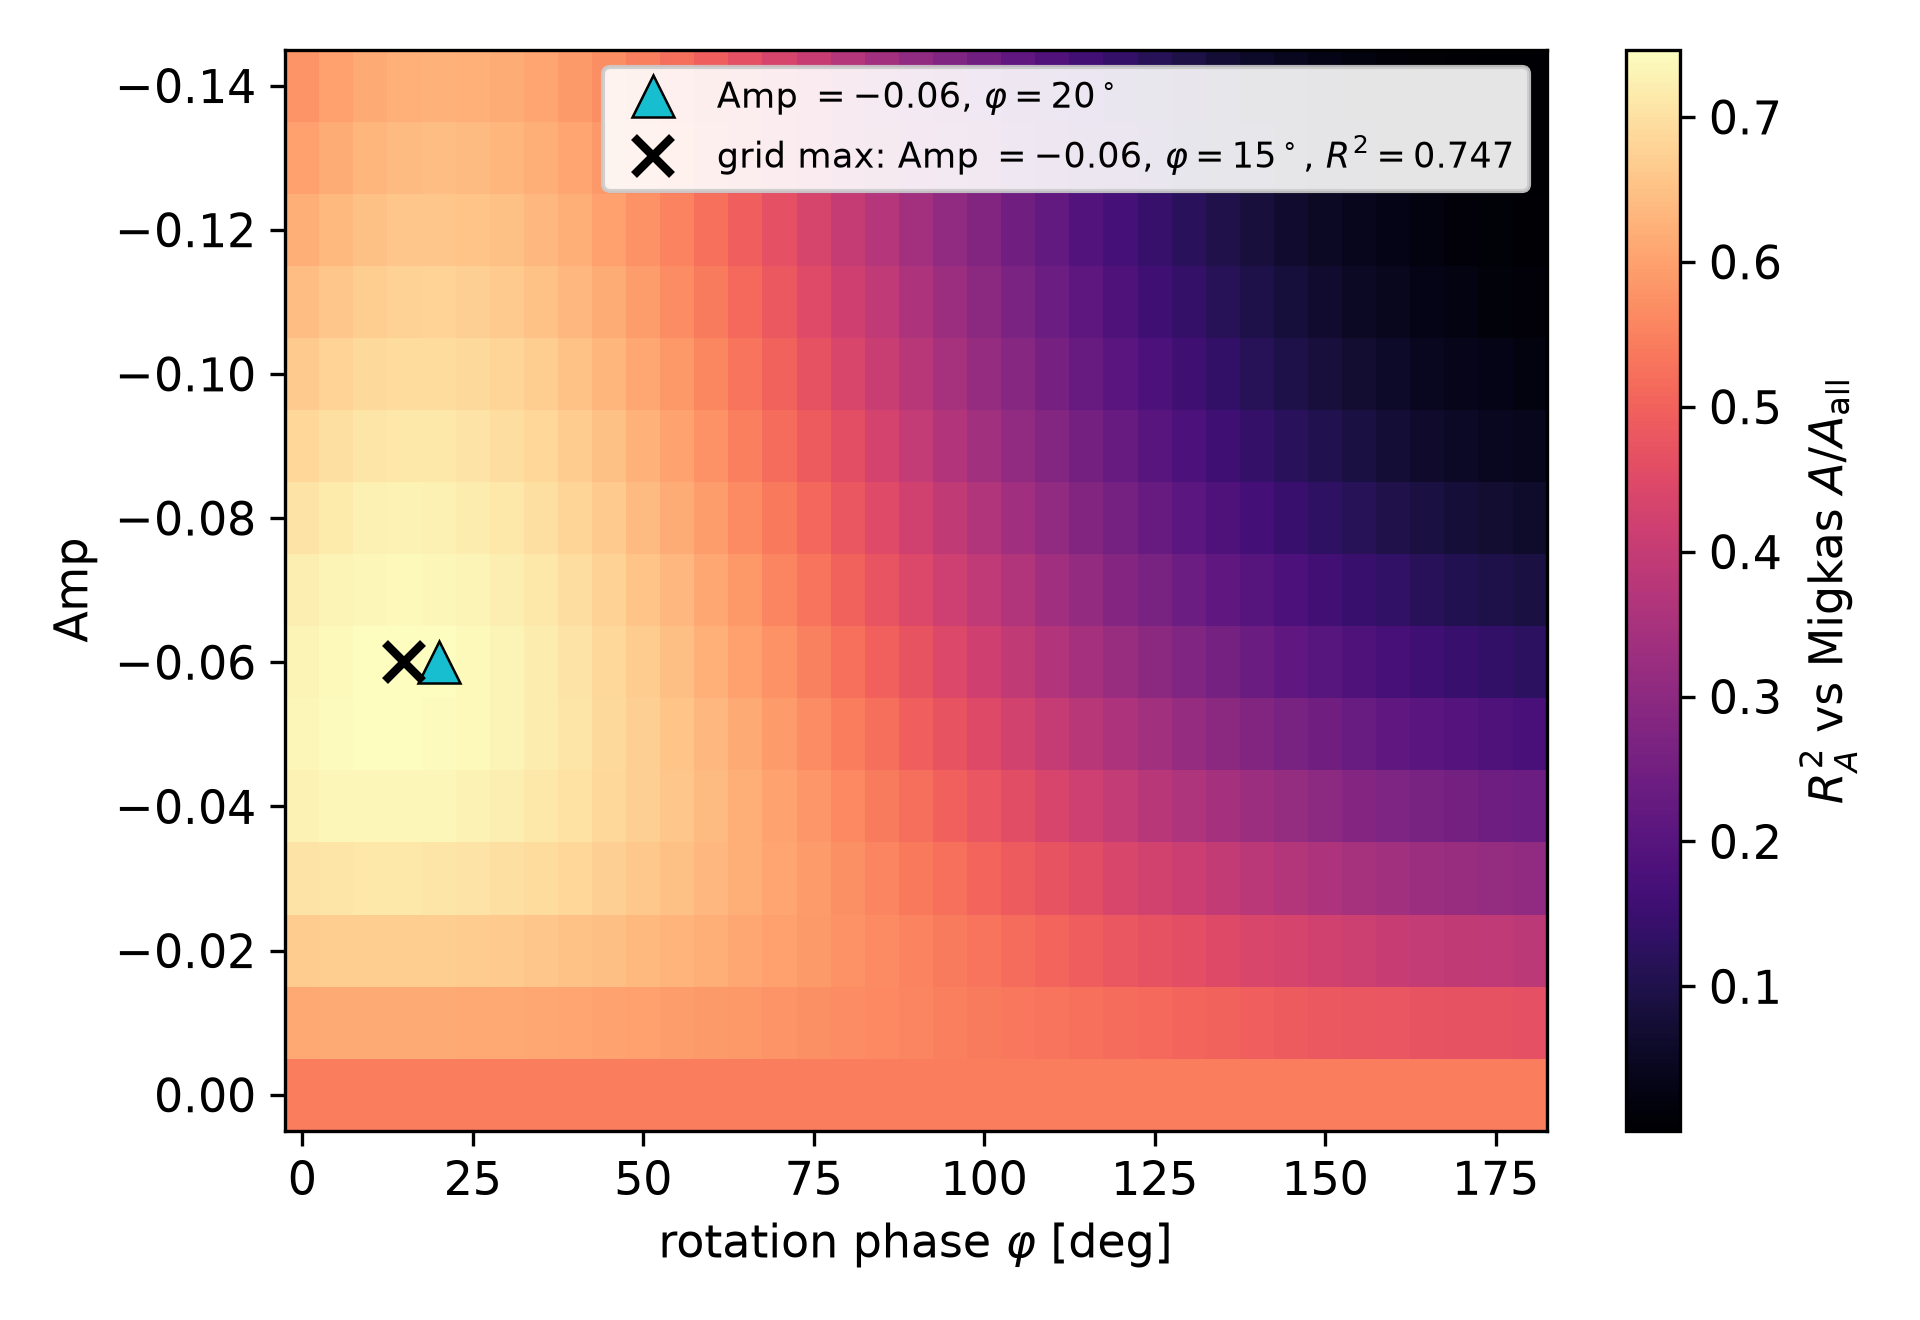
\includegraphics[width=\textwidth]{heatmap_R2_A_Amp_phi.png}
  \caption{$R^2_A$ versus Amp and $\varphi$.}
\end{subfigure}\hfill
\begin{subfigure}[t]{0.495\textwidth}
  \centering
  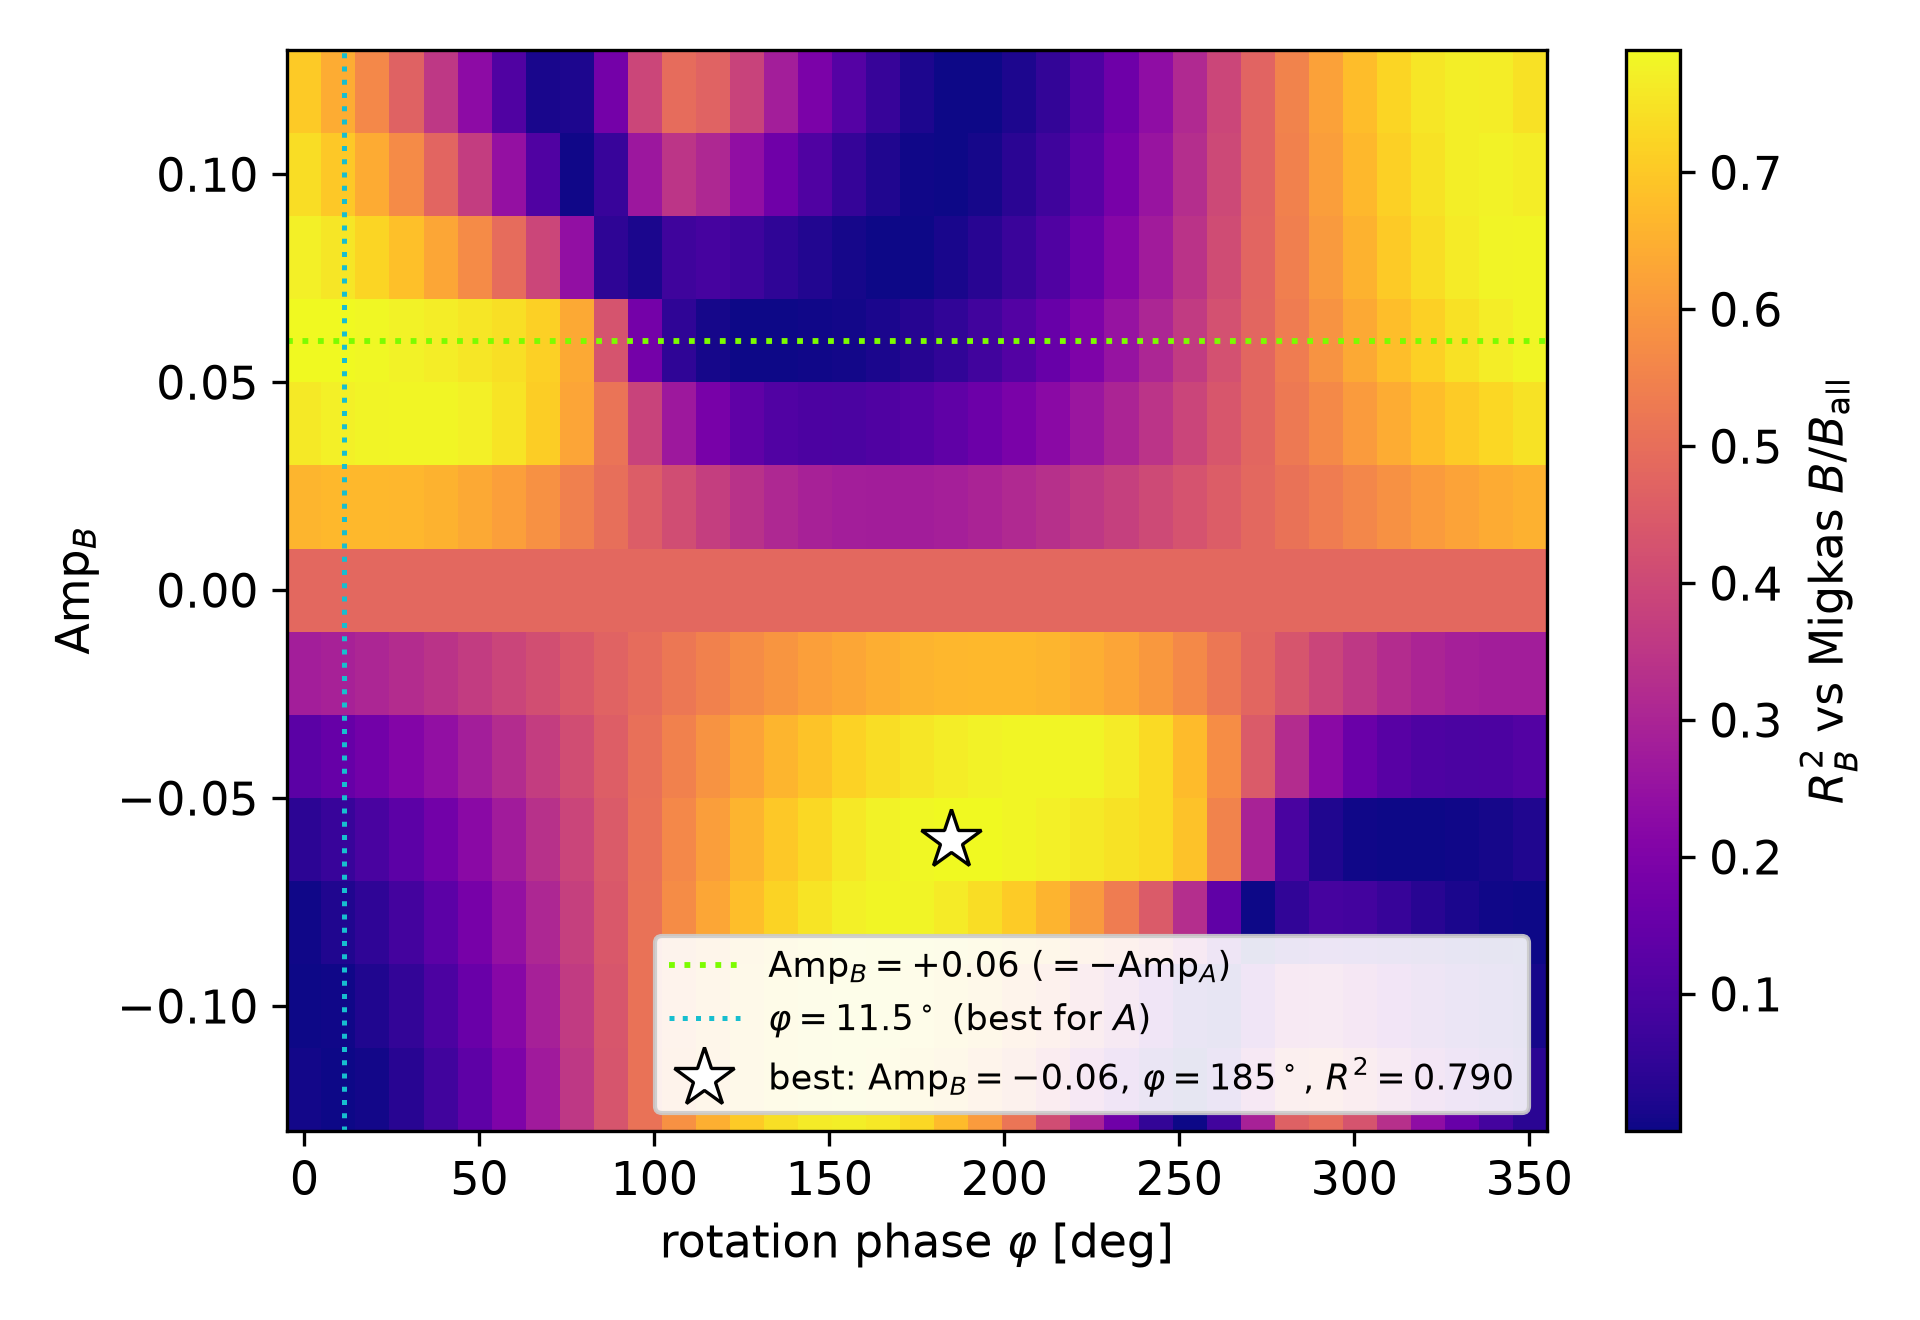
\includegraphics[width=\textwidth]{heatmap_R2_B_AmpB_phi.png}
  \caption{$R^2_B$ versus Amp$_B$ and $\varphi$.}
\end{subfigure}
\caption{Coefficient of determination of the phase-rotation template,
Eq.~\eqref{eq:ampsin}, as a function of amplitude and phase. (a)~$R^2_A$
against the Migkas et al.\ normalization profile $A/A_{\mathrm{all}}$ on a grid
of $\mathrm{Amp}\in[-0.14,0]$ (step $0.01$; axis inverted) and
$\varphi\in[0^\circ,180^\circ]$ (step $5^\circ$). The triangle marks
$\mathrm{Amp}=-0.06$, $\varphi=20^\circ$; the cross marks the grid maximum,
$R^2_A=0.747$ at $\mathrm{Amp}=-0.06$, $\varphi=15^\circ$. The best value from the
coarser parameter scan, $R^2_A=0.746$ at $\varphi=11.5^\circ$, lies on the same
ridge. (b)~$R^2_B$ against the slope profile $B/B_{\mathrm{all}}$ for an
independent amplitude $\mathrm{Amp}_B\in[-0.12,0.12]$ and
$\varphi\in[0^\circ,350^\circ]$. The star marks the best fit,
$R^2_B=0.790$ at $\mathrm{Amp}_B=-0.06$, $\varphi=185^\circ$; the dotted horizontal
line marks $\mathrm{Amp}_B=+0.06=-\mathrm{Amp}_A$ and the dotted vertical line
the phase $\varphi=11.5^\circ$ preferred by $A$.}
\label{fig:heatmaps}
\end{figure}

\begin{figure}[!htbp]
\centering
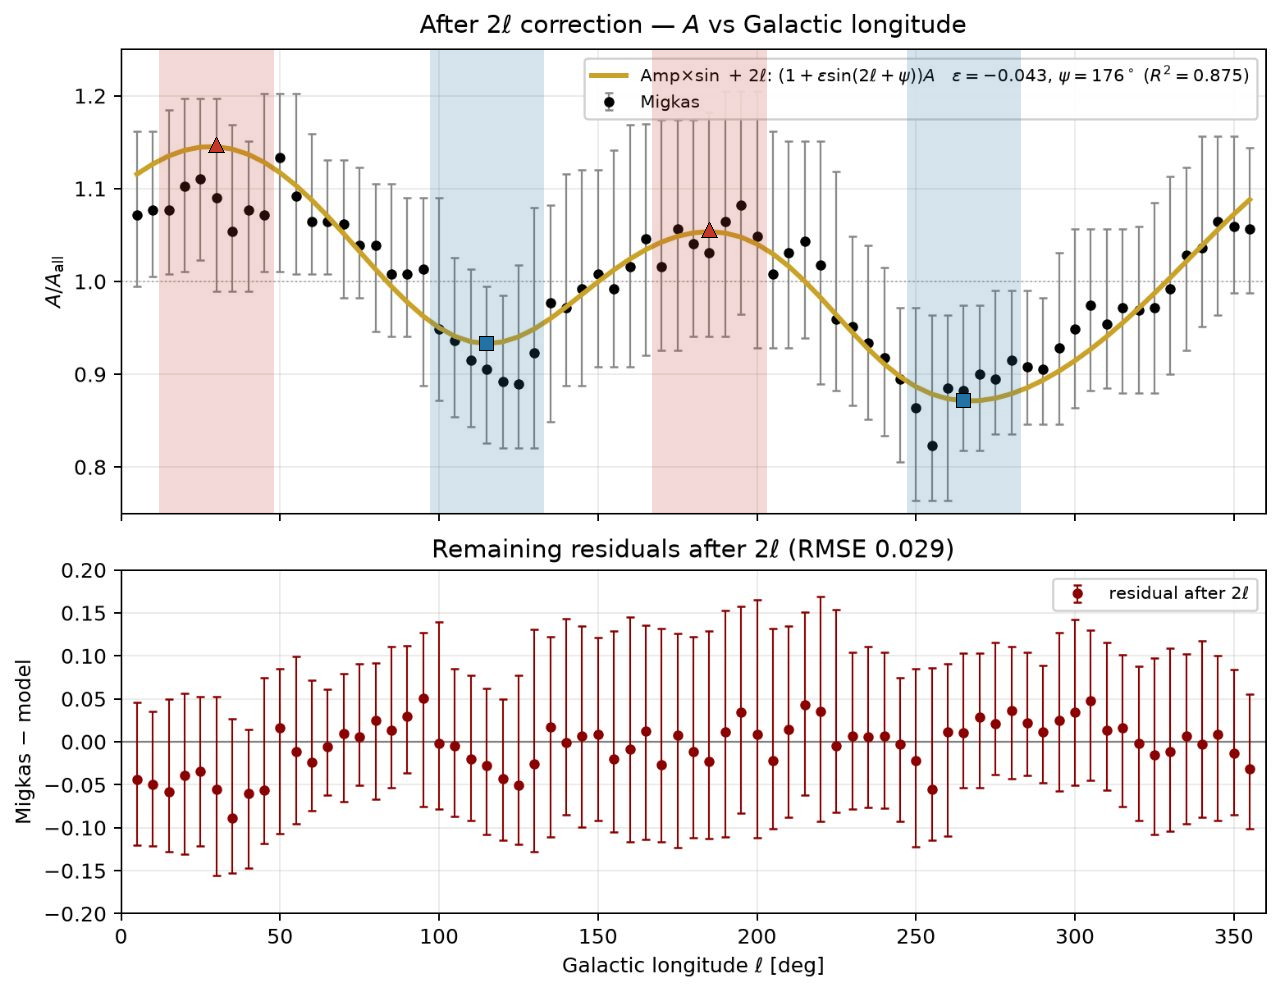
\includegraphics[width=0.85\textwidth]{A_vs_angle_after_2ell_with_residuals.png}
\caption{Model profile after the phase-rotation template and the
second-harmonic correction (Eqs.~\ref{eq:ampsin}--\ref{eq:2ell};
$\varepsilon=-0.043$, $\psi=176^\circ$), with $R^2=0.875$. Triangles and squares mark
the maxima ($\theta\simeq30^\circ,185^\circ$) and minima ($\theta\simeq115^\circ,265^\circ$);
shaded bands of $\pm18^\circ$ indicate their neighborhoods on the strip. Lower
panel: residuals (rms $0.029$).}
\label{fig:2ell}
\end{figure}

\begin{figure}[!htbp]
\centering
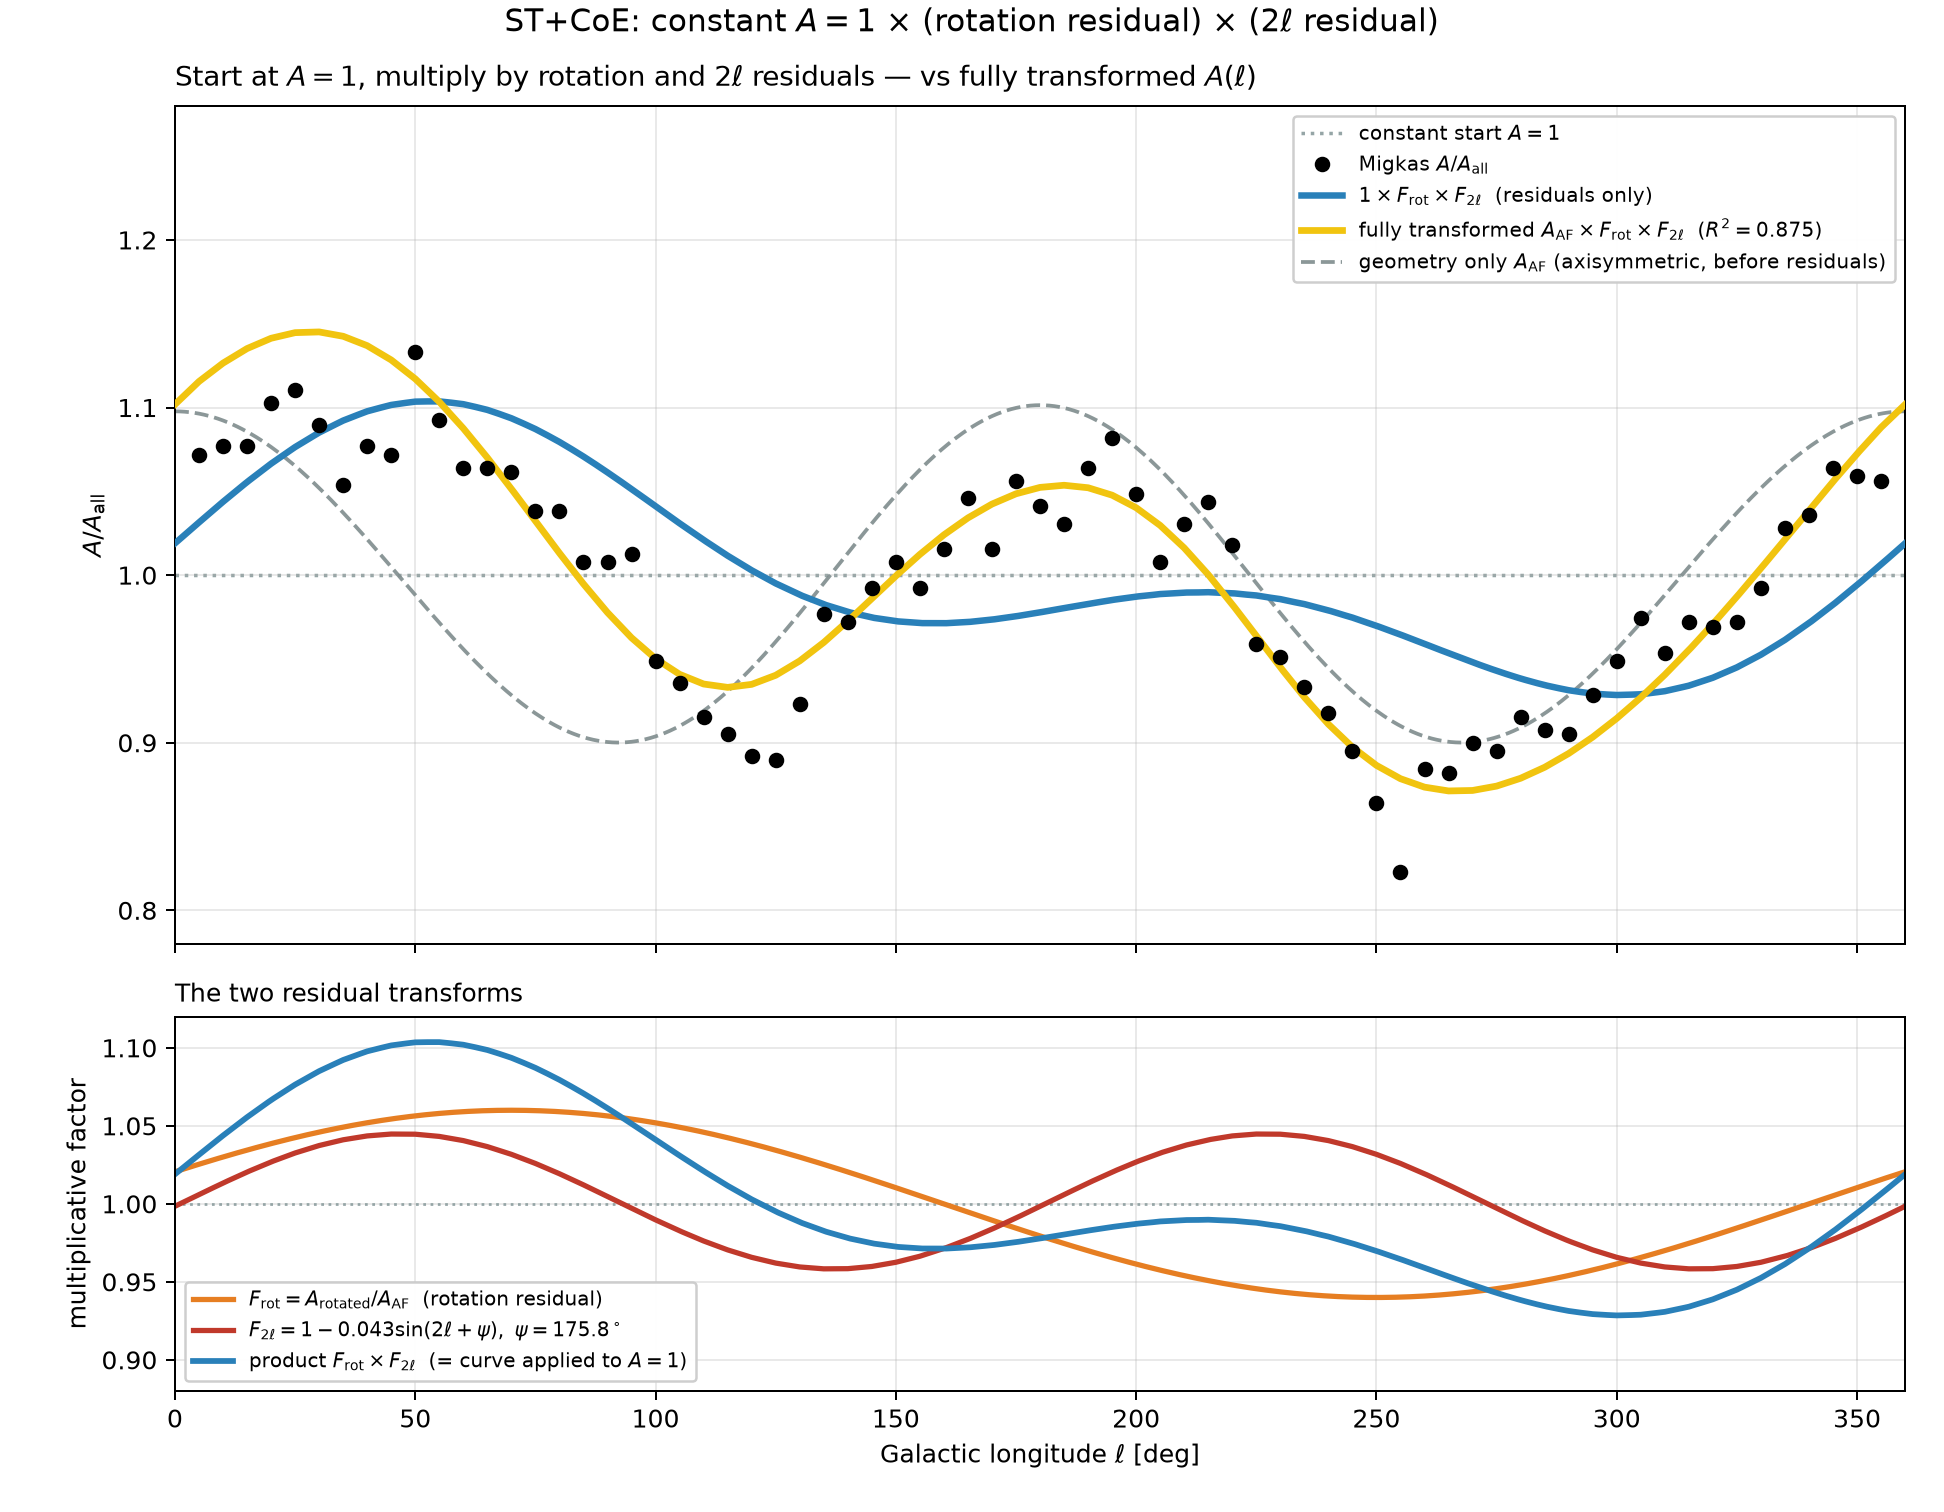
\includegraphics[width=0.85\textwidth]{A_from_constant_times_residuals_vs_full.png}
\caption{Decomposition of the corrected model. Upper panel: digitized data
(points), axisymmetric geometry alone (dashed), the correction factors applied
to a constant, $1\times F_{\mathrm{rot}}\times F_{2\ell}$ (blue; squared
correlation $0.366$), and the full model $A_{\mathrm{AF}}\times F_{\mathrm{rot}}
\times F_{2\ell}$ (yellow; $R^2=0.875$). Lower panel: the individual correction
factors and their product.}
\label{fig:resonly}
\end{figure}

\FloatBarrier
\subsection{Sky geometry of the extrema}

Figure~\ref{fig:halfrings} shows the four extremal angles mapped to rings about
the tilted CoE axis. Because the ring at angle $\theta$ and that at
$360^\circ-\theta$ coincide on the sky, the side of the axis on which the
$\theta$ ray lies is indicated by drawing only the half of each ring on that side
(the half satisfying $(\hat n\cdot\hat Y)\sin\theta\ge0$, where $\hat Y$ is the
in-plane direction perpendicular to the CoE axis). The angular radii of the
rings about the anti-CoE direction are $30^\circ$ (maximum), $175^\circ$ (maximum,
equivalently $5^\circ$ about the CoE), $115^\circ$ (minimum), and $95^\circ$ (minimum).

Figure~\ref{fig:halfmig} overlays the same half rings on the Migkas et al.\
$\theta=75^\circ$ map of $A/A_{\mathrm{all}}$. The highest-normalization direction
$(17^\circ,-9^\circ)$ lies $29.3^\circ$ from the anti-CoE direction, within $1^\circ$ of
the $\theta=30^\circ$ maximum ring, and the lowest-normalization direction
$(274^\circ,-22^\circ)$ lies $92.0^\circ$ from the anti-CoE direction, within $3^\circ$
of the $\theta=265^\circ$ minimum ring (angular radius $95^\circ$); both fall inside
the $\pm9^\circ$ bands. The secondary extrema of the longitude profile, marked on
the Galactic plane, behave differently: $(115^\circ,0^\circ)$ lies $114.1^\circ$ from the
anti-CoE direction, on the $\theta=115^\circ$ minimum ring, whereas $(185^\circ,0^\circ)$
lies $164.2^\circ$ from it, $11^\circ$ from the center line of the $\theta=185^\circ$
maximum ring and just outside its band.

Figures~\ref{fig:gradrings} and~\ref{fig:gradmig} show the same geometry with
full rings. The opacity of each ring decreases linearly with azimuth $\psi$
around the ring, measured from the point on the $\theta$-ray side,
$\alpha\propto1-0.88\,|\psi|/\pi$, so that each ring is darkest where the $\theta$
ray meets it and falls to $12\%$ opacity at the diametrically opposite point.
This representation shows the complete small circles while retaining the
side information of the half-ring figures.

\begin{figure}[!htbp]
\centering
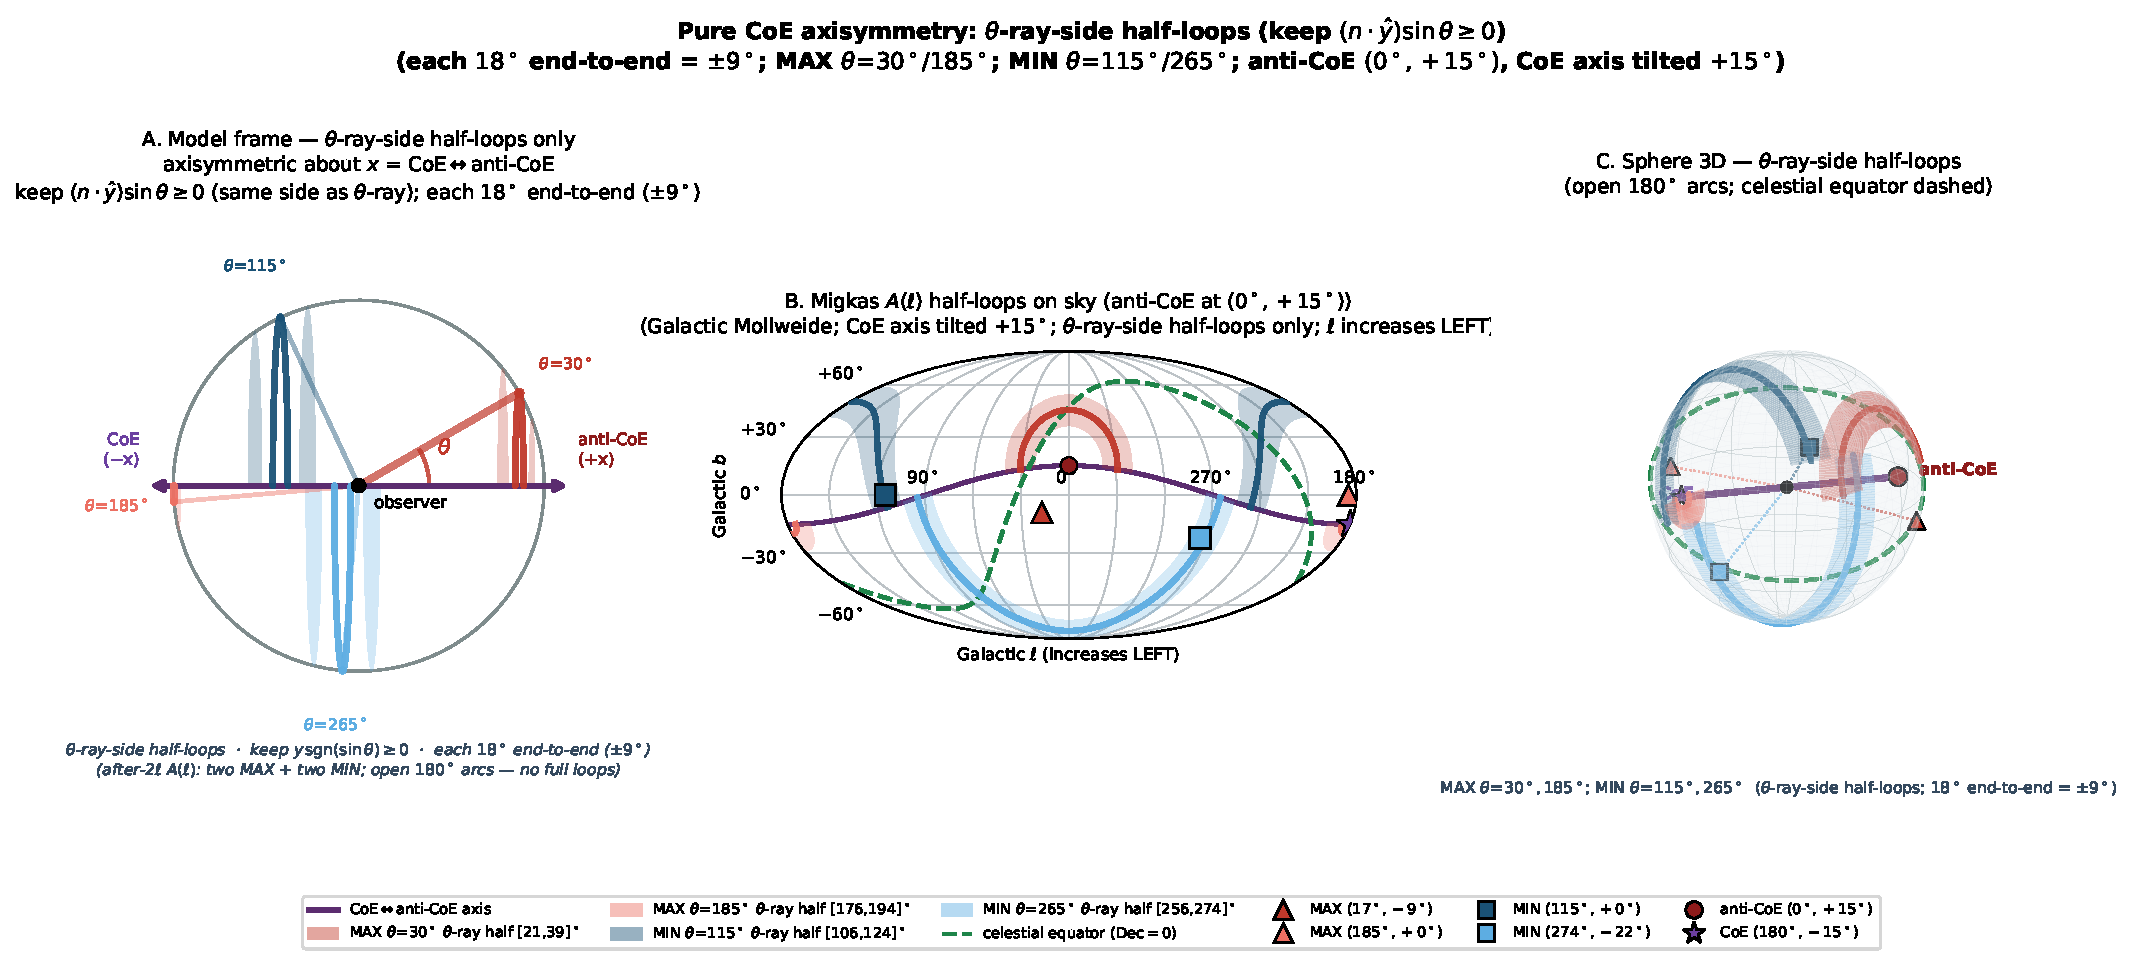
\includegraphics[width=\textwidth]{coe_rings_half_loops_tilt15_theta_ray_side.pdf}
\caption{Sky geometry of the four extrema of the corrected longitude profile,
with the CoE axis tilted by $+15^\circ$ (anti-CoE at $(\ell,b)=(0^\circ,+15^\circ)$, CoE
at $(180^\circ,-15^\circ)$). Maxima at $\theta=30^\circ$ and $185^\circ$ (red) and minima at
$\theta=115^\circ$ and $265^\circ$ (blue), measured from the anti-CoE direction, each
with a band of $\pm9^\circ$. Only the half of each ring on the side of its $\theta$
ray is drawn. (A)~Model frame, axisymmetric about the CoE--anti-CoE axis.
(B)~Galactic Mollweide projection, longitude increasing to the left; the dashed
curve is the celestial equator. (C)~Three-dimensional view of the celestial
sphere. Triangles and squares mark the reference maxima at $(17^\circ,-9^\circ)$,
$(185^\circ,0^\circ)$ and minima at $(115^\circ,0^\circ)$, $(274^\circ,-22^\circ)$.}
\label{fig:halfrings}
\end{figure}

\begin{figure}[!htbp]
\centering
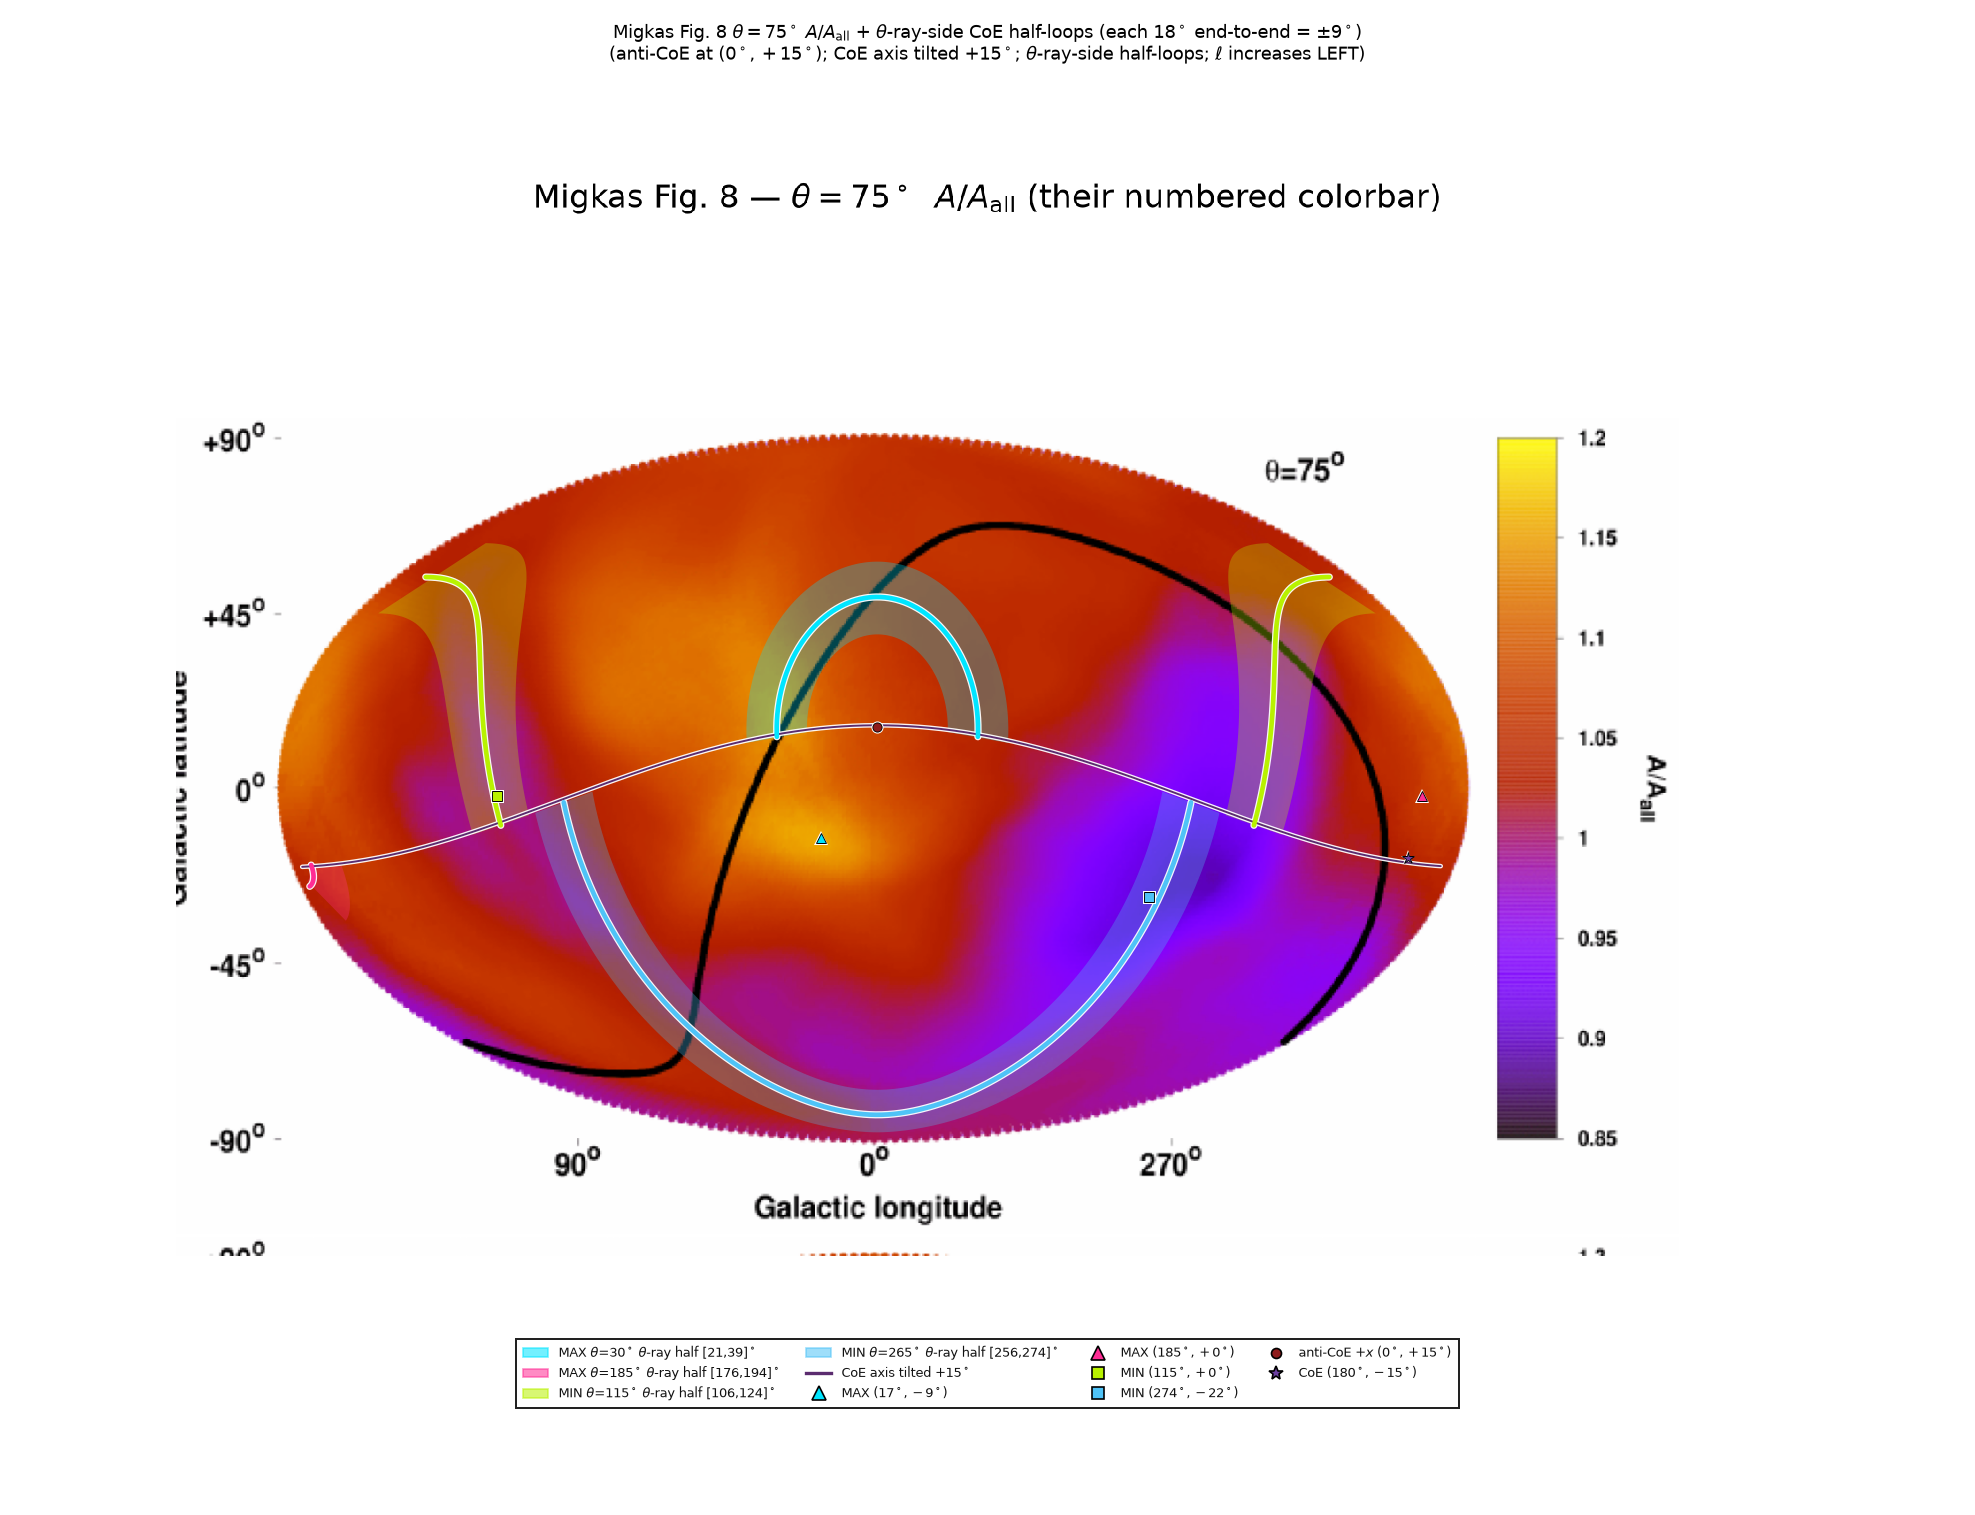
\includegraphics[width=0.88\textwidth]{migkas_fig8_half_loops_tilt15_theta_ray_side.png}
\caption{Half rings of Fig.~\ref{fig:halfrings} overlaid on the
$\theta=75^\circ$ map of $A/A_{\mathrm{all}}$ from Migkas et al.~\citep{Migkas2020}
(their Fig.~8, reproduced with its original color scale). CoE axis tilted by
$+15^\circ$ (white-outlined line). Markers:
maxima at $(17^\circ,-9^\circ)$ and $(185^\circ,0^\circ)$; minima at $(115^\circ,0^\circ)$ and
$(274^\circ,-22^\circ)$.}
\label{fig:halfmig}
\end{figure}

\begin{figure}[!htbp]
\centering
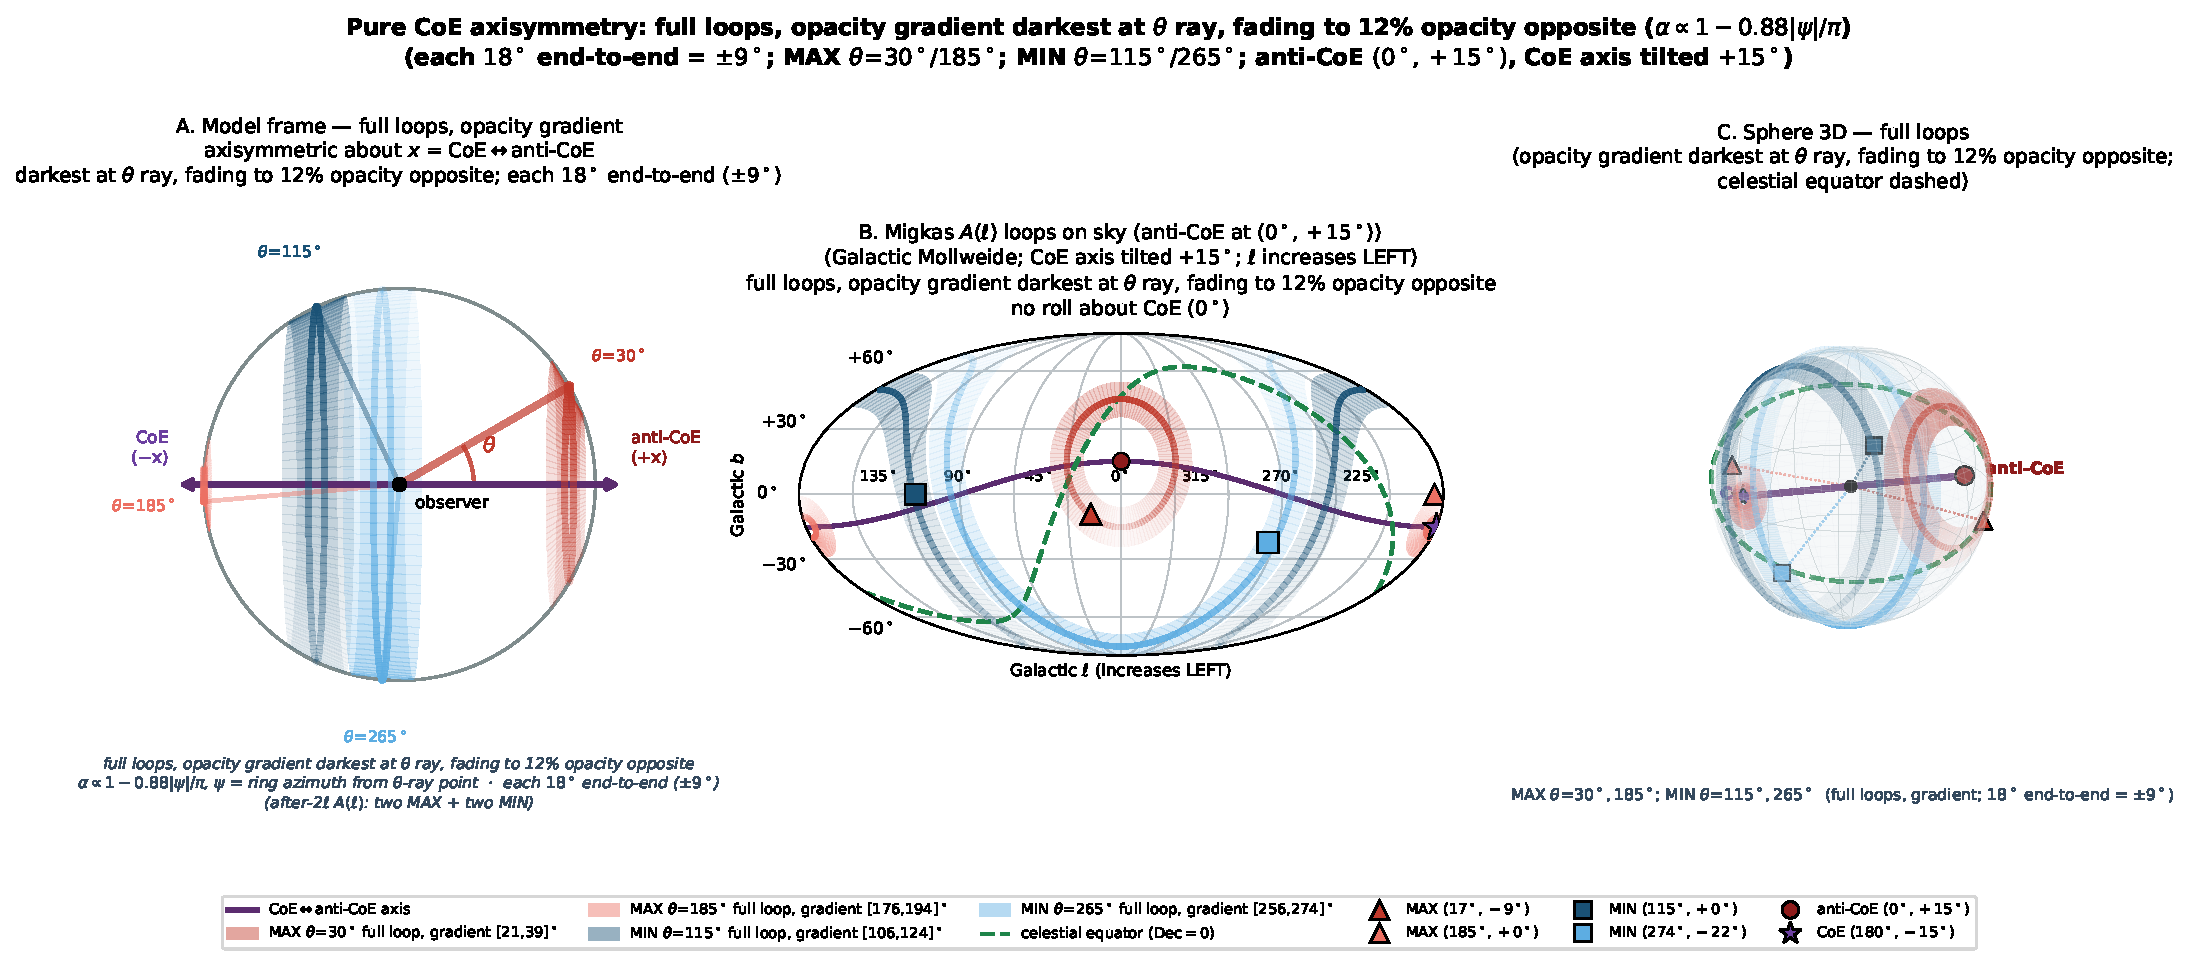
\includegraphics[width=\textwidth]{coe_rings_gradient_loops_tilt15.pdf}
\caption{As Fig.~\ref{fig:halfrings}, but showing the full rings with an
opacity gradient: each ring is darkest at the point on the side of its $\theta$
ray and fades linearly in azimuth to $12\%$ opacity at the opposite point
($\alpha\propto1-0.88\,|\psi|/\pi$). Anti-CoE at $(0^\circ,+15^\circ)$, CoE at
$(180^\circ,-15^\circ)$; maxima at $\theta=30^\circ,185^\circ$ and minima at
$\theta=115^\circ,265^\circ$, each $\pm9^\circ$ wide. Panels (A)--(C) as in
Fig.~\ref{fig:halfrings}.}
\label{fig:gradrings}
\end{figure}

\begin{figure}[!htbp]
\centering
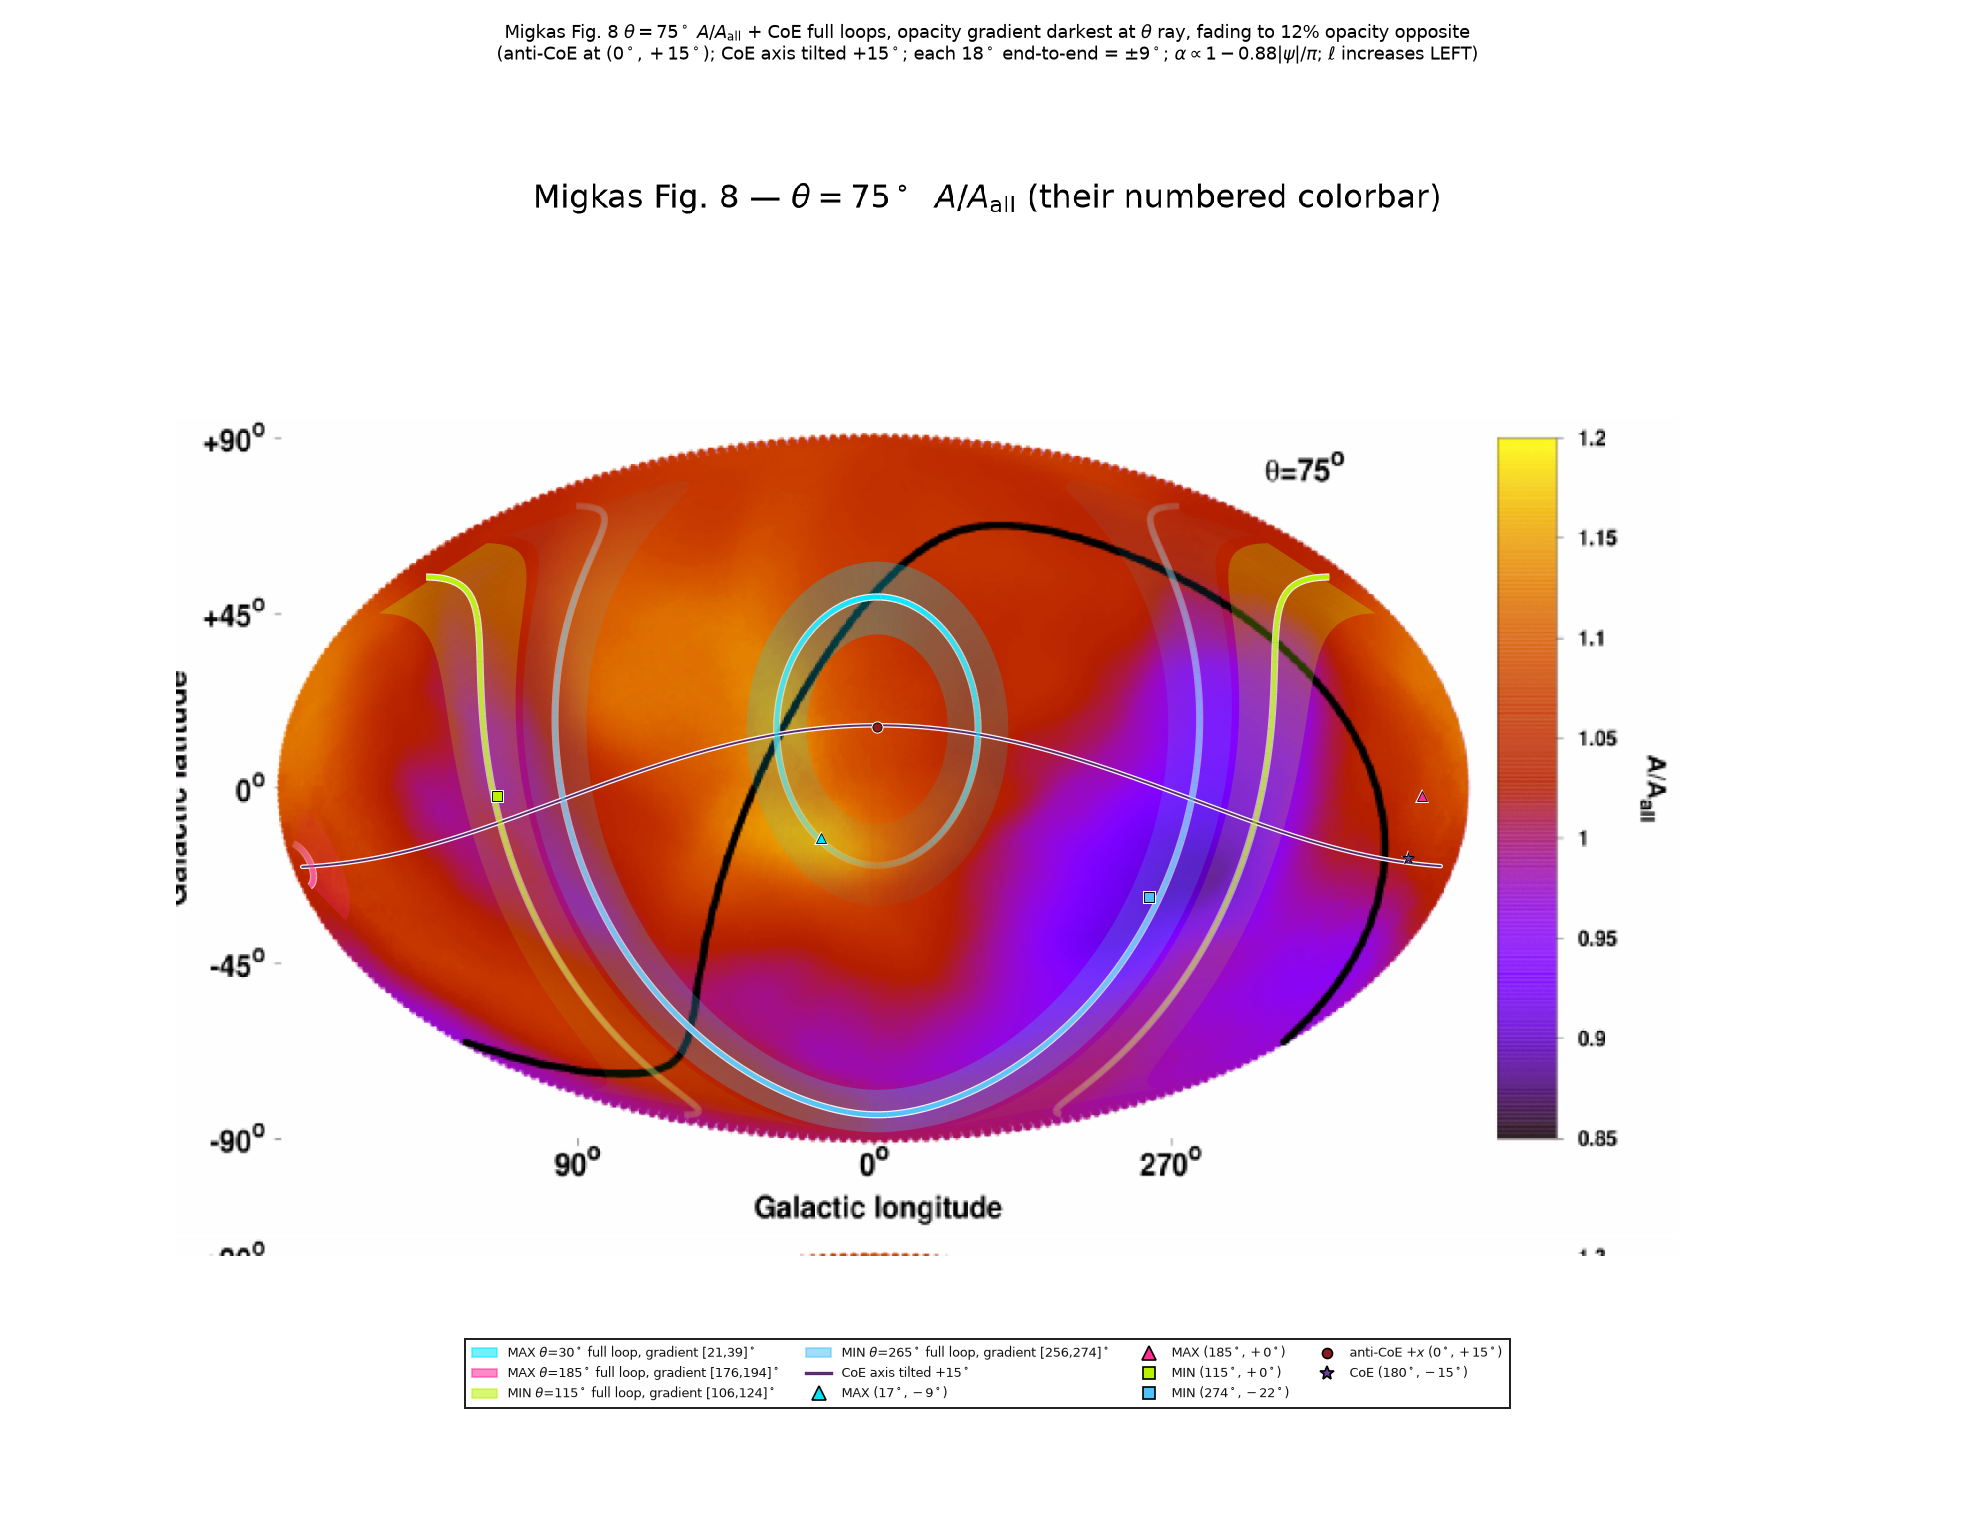
\includegraphics[width=0.88\textwidth]{migkas_fig8_gradient_loops_tilt15.png}
\caption{Full rings of Fig.~\ref{fig:gradrings}, with the same opacity gradient,
overlaid on the Migkas et al.~\citep{Migkas2020} $\theta=75^\circ$ map of
$A/A_{\mathrm{all}}$. Markers as in Fig.~\ref{fig:halfmig}.}
\label{fig:gradmig}
\end{figure}

\FloatBarrier
The orientation of the rings about the CoE axis is not fixed by the
axisymmetric model in the model frame; only the axis direction is. As an
illustration of the effect of this freedom on the sky projection,
Fig.~\ref{fig:rot45} shows the full-ring geometry with the sky panels rolled by
$45^\circ$ counter-clockwise about the CoE axis, the model-frame panel being left
unchanged.

\begin{figure}[!htbp]
\centering
\begin{subfigure}{\textwidth}
  \centering
  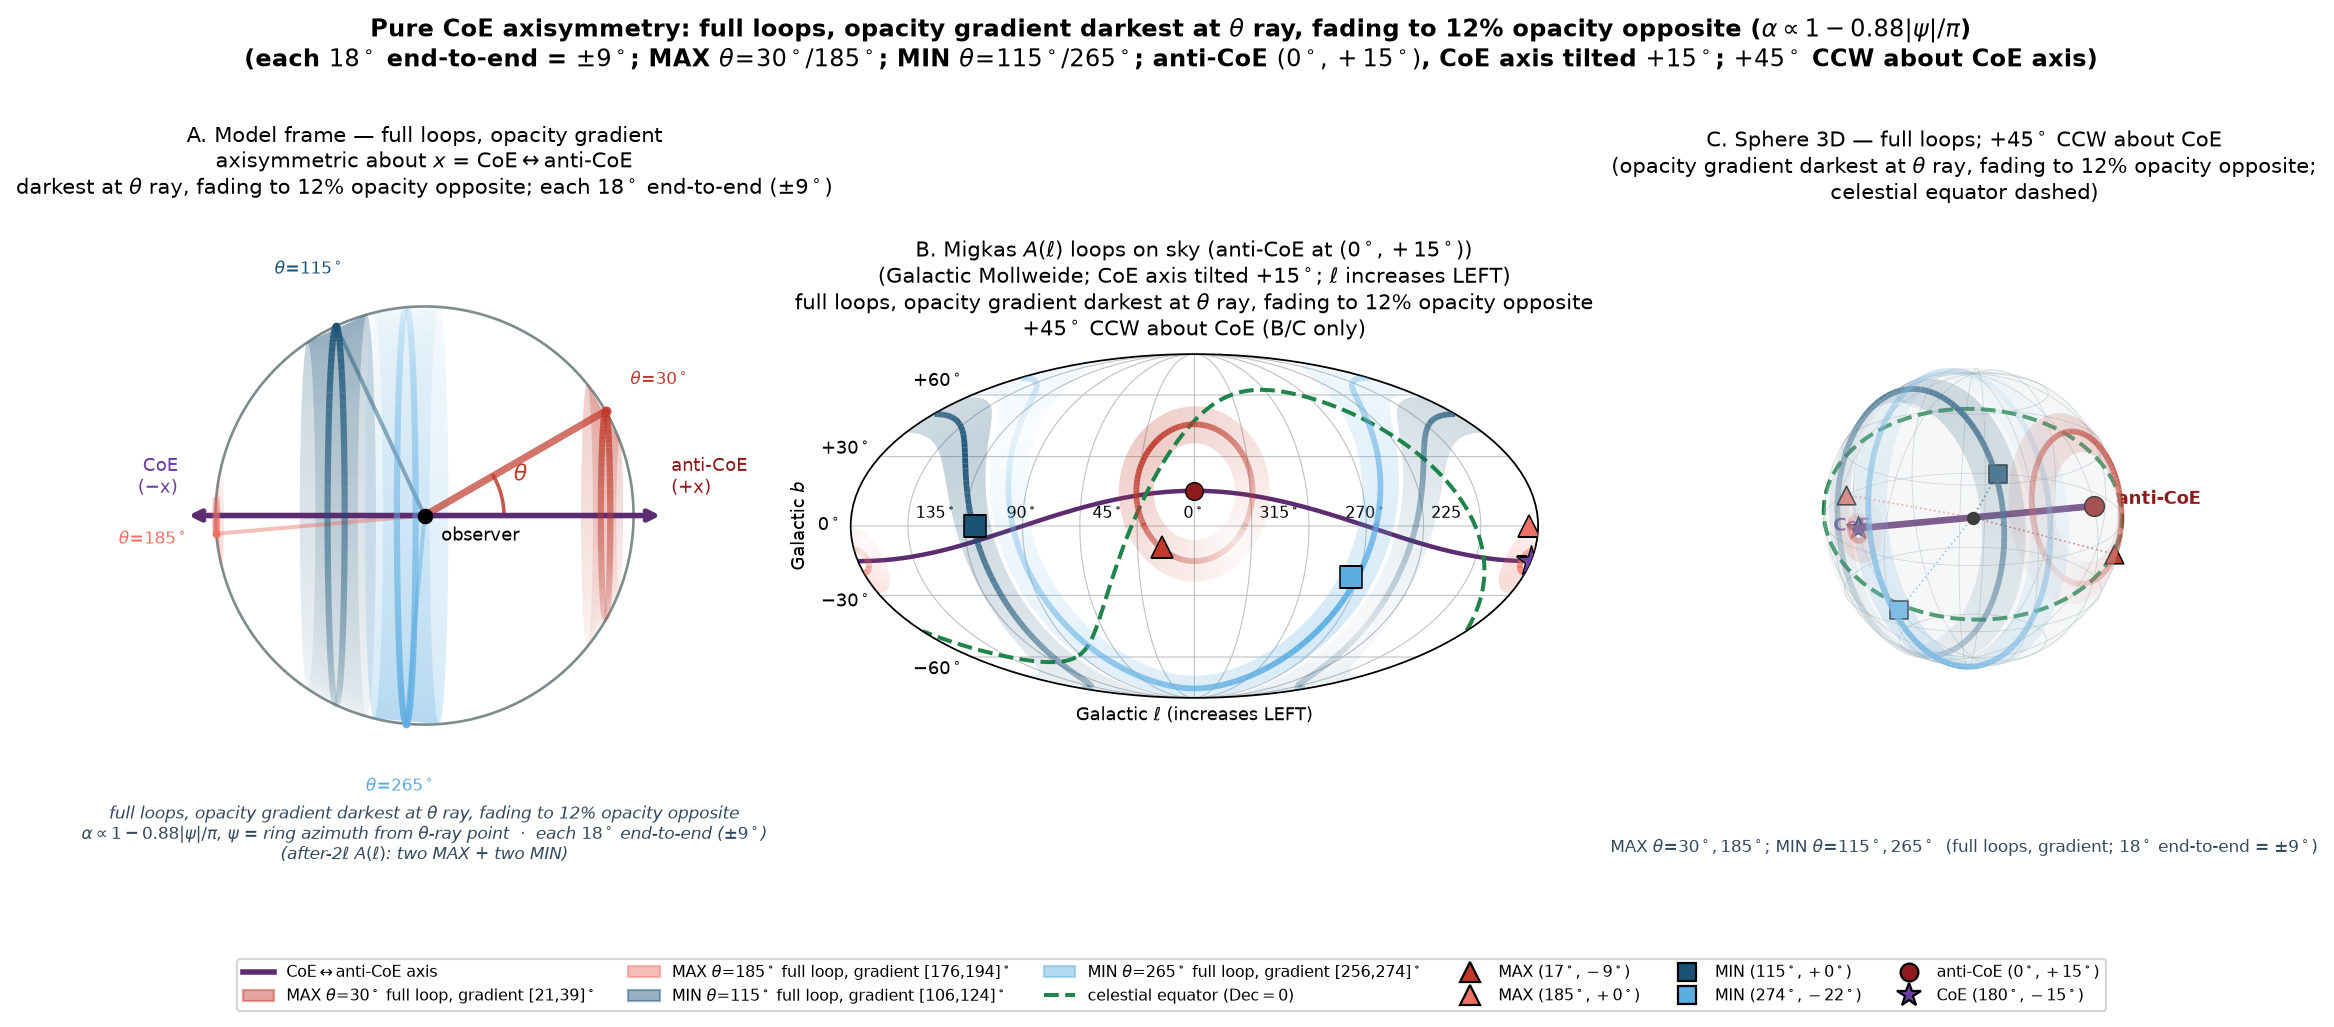
\includegraphics[width=\textwidth]{coe_rings_gradient_loops_tilt15_rot45ccw.png}
  \caption{Three-panel geometry; panels B and C rolled by $45^\circ$
  counter-clockwise about the CoE axis, panel A unrolled.}
\end{subfigure}\\[0.6em]
\begin{subfigure}{0.72\textwidth}
  \centering
  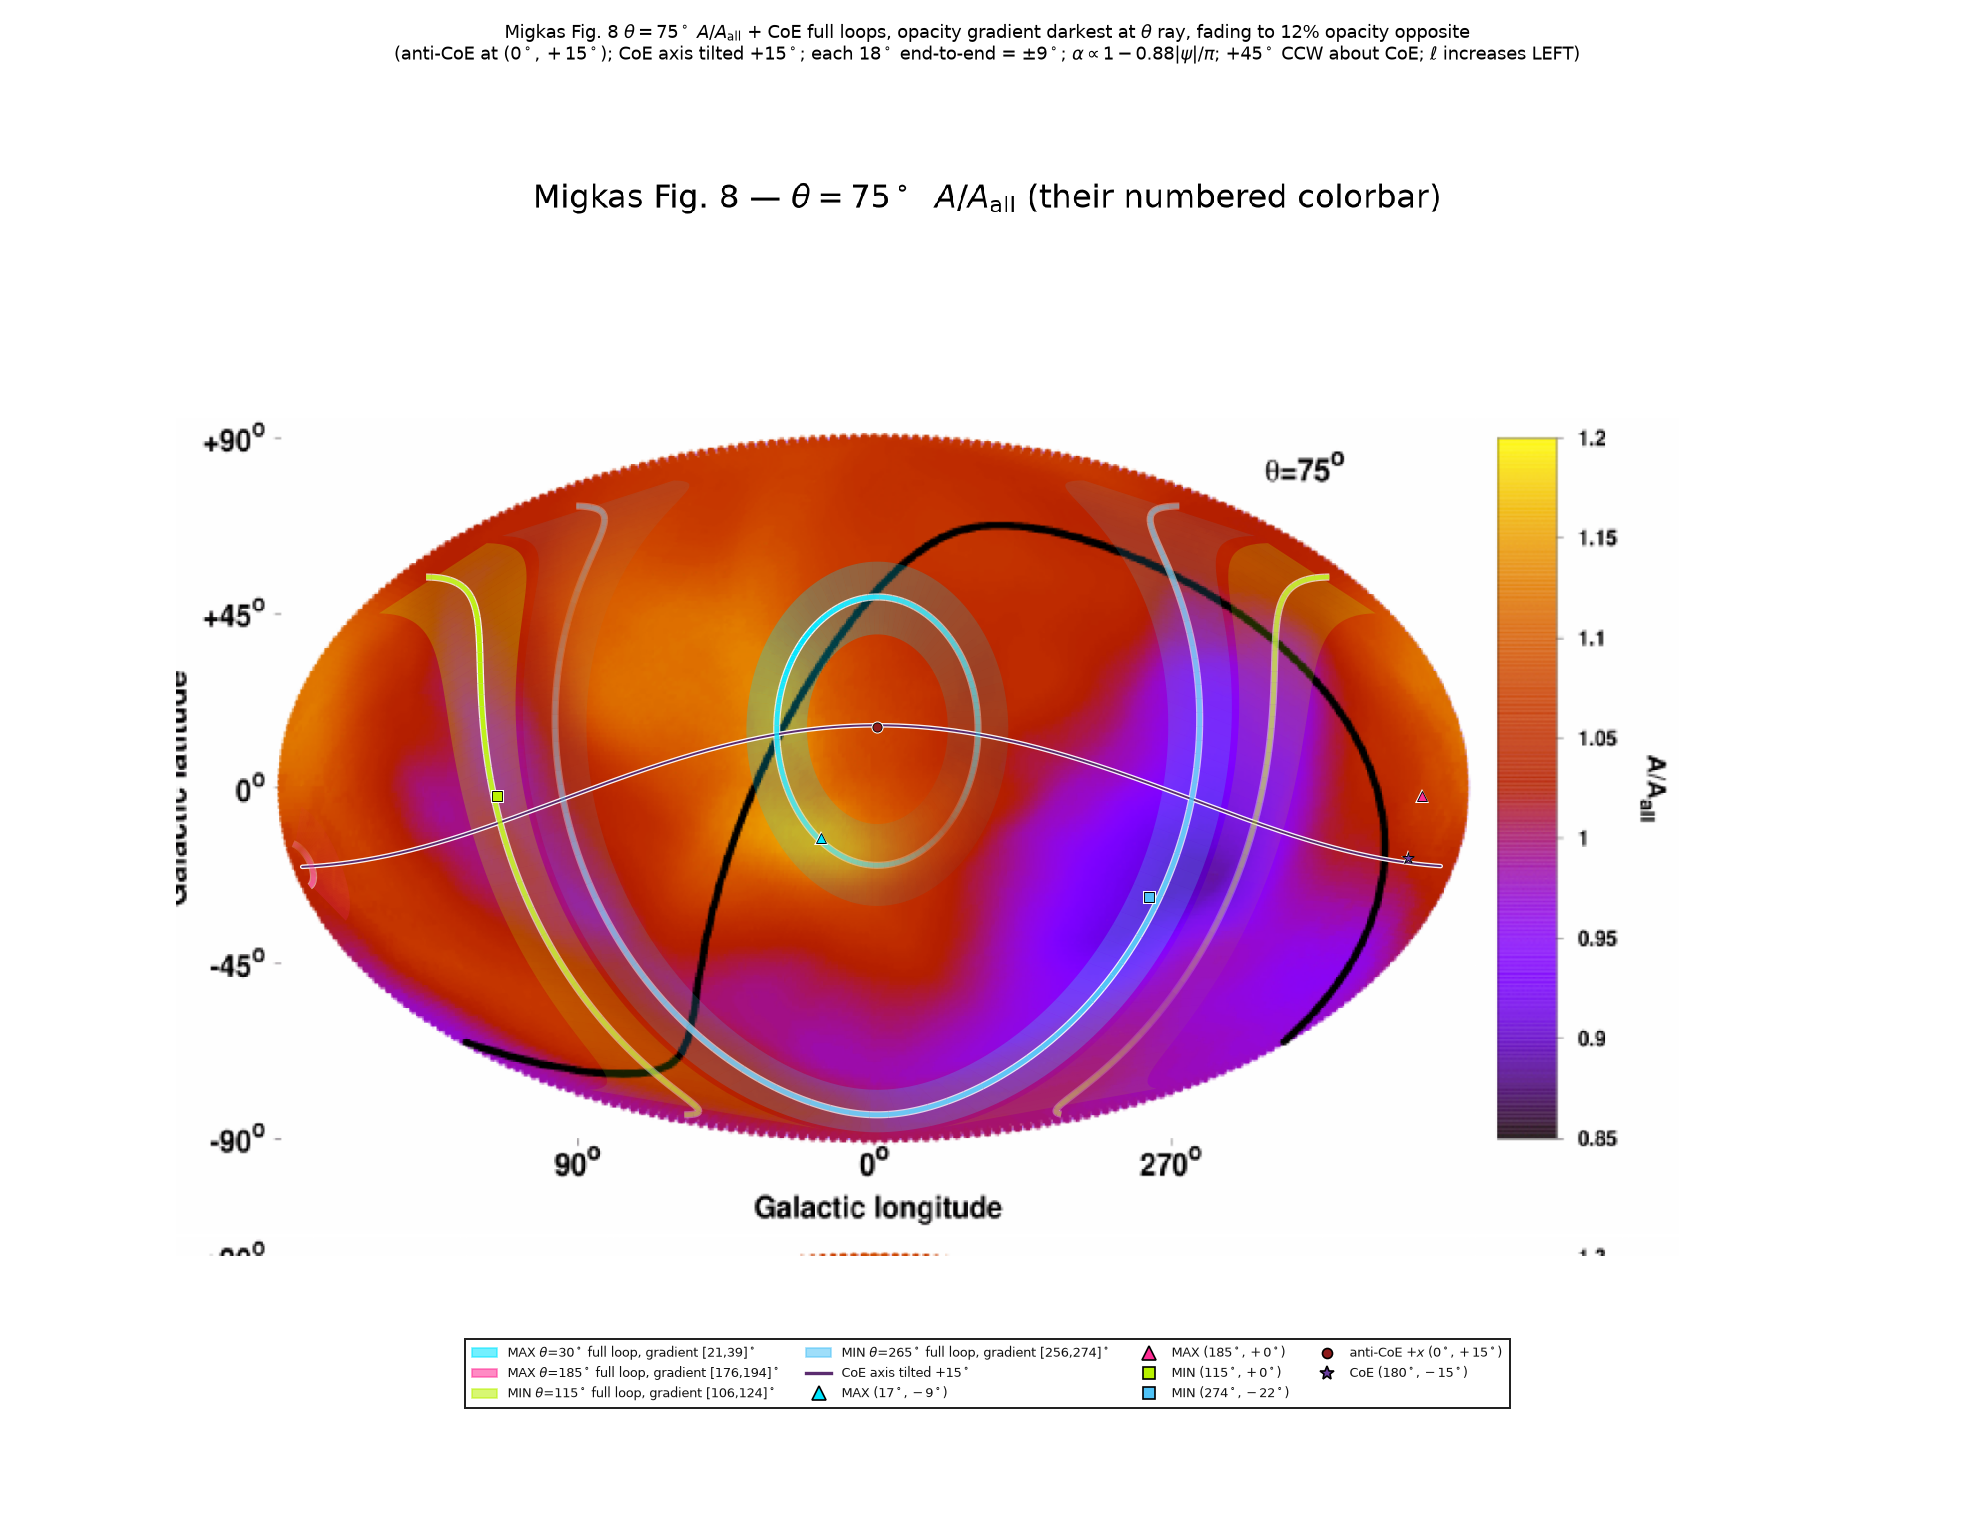
\includegraphics[width=\textwidth]{migkas_fig8_gradient_loops_tilt15_rot45ccw.png}
  \caption{Overlay on the Migkas et al.\ $\theta=75^\circ$ map with the same roll.}
\end{subfigure}
\caption{Full-ring geometry of Figs.~\ref{fig:gradrings}
and~\ref{fig:gradmig} with the sky projection rolled by $45^\circ$
counter-clockwise about the CoE axis (anti-CoE at $(0^\circ,+15^\circ)$, CoE at
$(180^\circ,-15^\circ)$).}
\label{fig:rot45}
\end{figure}

\FloatBarrier
%======================================================================
\section{Discussion}
\label{sec:discussion}

\paragraph{Origin of the anisotropy.}
A central result of the model is that the displacement of the observer from
the CoE is, by itself, unobservable in relative velocities: homologous
expansion yields the same $H$ in every direction for every observer
(Eq.~\ref{eq:Hobs}). Direction dependence is produced by the enclosed-mass
gravity of a decreasing density profile, and at leading order it takes the
form of a quadrupole about the CoE axis (Eq.~\ref{eq:tidal}). The empirical
finding that the second harmonic dominates the Migkas et al.\ longitude
profile (Eq.~\ref{eq:dq}) is consistent with this structure. A pure dipole
description, by contrast, accounts for only about a quarter of the variance.

\paragraph{Status of the templates.}
The phase-rotation template (Eq.~\ref{eq:ampsin}) and the second-harmonic
correction (Eq.~\ref{eq:2ell}) are introduced empirically and are not yet
derived from the time-integrated enclosed-mass acceleration. Their parameters
are fitted to the same data used to evaluate the agreement, so the improvement
from $R^2=0.307$ to $R^2=0.875$ should not be regarded as a test of the model.
The decomposition of Fig.~\ref{fig:resonly} indicates that the correction
factors alone account for a minority of the variance, but a first-principles
derivation of any departure from axisymmetry---for example from a
non-spherical mass distribution or from the time dependence of the flow---is
required before the corrected profile can be regarded as a prediction.

\paragraph{Sky geometry.}
The ring construction translates the longitude profile into a
two-dimensional prediction that can be compared with the Migkas et al.\ sky
map. With the CoE axis tilted by $15^\circ$, the principal maximum and minimum
rings pass close to the published extrema, while the ring associated with the secondary maximum
at $(185^\circ,0^\circ)$ is offset by about $11^\circ$. The comparison is at present
qualitative; a quantitative test requires evaluating the model on the full
sky with the survey footprint and cone-averaging used by Migkas et al., and
assessing the significance of the alignment against randomly oriented axes.

\paragraph{Relation to the cosmic microwave background.}
The present work addresses the late-universe anisotropy of the Hubble flow
as traced by the X-ray cluster scaling relation. A quantitative comparison with
the cosmic microwave background, including its dipole and low multipoles,
within the full model is deferred to future work. No conflict with CMB data is
asserted or demonstrated here, and consistency is likewise not claimed.

\paragraph{Relativistic generalization.}
The dynamics have been treated in the Newtonian Sedov--Taylor limit with
homologous interior flow. The relativistic blast-wave solutions of Blandford
and McKee~\citep{BlandfordMcKee1976}, the cosmological self-similar shocks of
Bertschinger~\citep{Bertschinger1983}, and the general-relativistic shock-wave
cosmologies of Smoller and Temple~\citep{SmollerTemple2000,SmollerTemple2003}
provide the frameworks within which the model can be extended to relativistic
velocities and to distances comparable to or beyond the Hubble length, where
the CoE is assumed to lie.

%======================================================================
\section{Conclusions}
\label{sec:conclusions}

We have described a model in which the cosmic expansion is the interior flow of
a Sedov--Taylor self-similar blast wave, $R\propto t^{2/(5-w)}$ for an ambient
density $\rho\propto r^{-w}$, launched from a Center of Expansion beyond the
horizon. Our conclusions are as follows.
\begin{enumerate}
\item Homologous expansion gives an isotropic apparent Hubble law for any
  observer, independent of the observer's distance from the CoE.
\item Enclosed-mass gravity, $g=-GM(<r)/r^2$, in a centrally concentrated,
  outward-decreasing density profile breaks homology and produces a
  direction-dependent $H_{\mathrm{obs}}$ whose leading term is a quadrupole about
  the CoE axis, with natural strength $\kappa=\Omega_m/2=0.15$.
\item The Migkas et al.\ $A(\ell)$ profile is dominated by its second harmonic:
  a dipole-plus-quadrupole fit gives $R^2=0.814$ against $0.271$ for a dipole
  alone.
\item The axisymmetric model gives $R^2=0.307$; with empirical phase-rotation and
  second-harmonic corrections the agreement reaches $R^2=0.875$.
\item Mapped onto the sky about a CoE axis tilted by $15^\circ$, with the
  anti-CoE direction at $(0^\circ,+15^\circ)$, the principal extremal rings pass
  within a few degrees of the published maximum and minimum of the $A$ map.
\end{enumerate}
The next steps are a first-principles derivation of the corrections from
time-integrated gravity, a full-sky comparison including the survey footprint,
and a quantitative treatment of the cosmic microwave background within the
model.

\section*{Acknowledgments}
The author thanks Wolfgang Rindler and Luke Ackerman for the early discussions
in which the Sedov--Taylor centered-universe idea was developed. The sky maps
in Figs.~\ref{fig:halfmig}, \ref{fig:gradmig} and~\ref{fig:rot45} use the
$\theta=75^\circ$ normalization map published by Migkas et al.~\citep{Migkas2020}.

\bibliographystyle{unsrtnat}
\bibliography{refs}

\end{document}
